\documentclass[11pt]{article}

\usepackage[T1]{fontenc}
\usepackage[polish]{babel}
\usepackage[utf8]{inputenc}
\usepackage{lmodern}
\selectlanguage{polish}

\title{Komunikacja Człowiek-Komputer \newline rozpoznawanie nut}
\author{Kuba Wąsik (132335), Dominik Szmyt (132326)}
\date{18.11.2018}

\usepackage{natbib}
\usepackage{graphicx}
\usepackage{subcaption}
\usepackage{float}

\begin{document}

\maketitle

\section{Zastosowanie}


Program służy do wykrywania nut ze zdjęcia.
Jest w stanie odnaleźć klucze (wiolinowy i basowy) oraz wypisać kolejność pojawienia się nuty, jej wysokość oraz numer pięciolinii, w której się znajduje.  

\section{Przetwarzanie}

Opiszemy najważniejsze kroki, jakie podjęliśmy, aby wykryć nuty.

\subsection{Wycinanie strony}

Pierwszym krokiem, który należało wykonać było "wyłuskanie" ~ ze zdjęcia samej kartki. 
W tym celu poszukiwaliśmy największego konturu na obrazie, który ma cztery narożniki, zakładając, że to nasza kartka. 
Aby było to możliwe, wcześniej nakładaliśmy filtr Canny. 
Kiedy już odnaleźliśmy nasze narożniki, po odpowiednim ich posortowaniu używaliśmy dla nich funkcji \textbf{cv2.getPerspectiveTransform()}
oraz \textbf{cv2.warpPerspective()}, aby odpowiednio znaleźć macierz transformacji i zastosować ją na zdjęciu. 

\begin{figure}
    \centering
    \begin{subfigure}{.5\textwidth}
        \centering
        \graphicspath{ {Resources/} }
        \includegraphics[width=.9\linewidth]{nutki_04.jpg}
        % \caption{A subfigure}
        \label{fig:sub1}
    \end{subfigure}%
    \begin{subfigure}{.5\textwidth}
        \centering
        \graphicspath{ {output/} }
        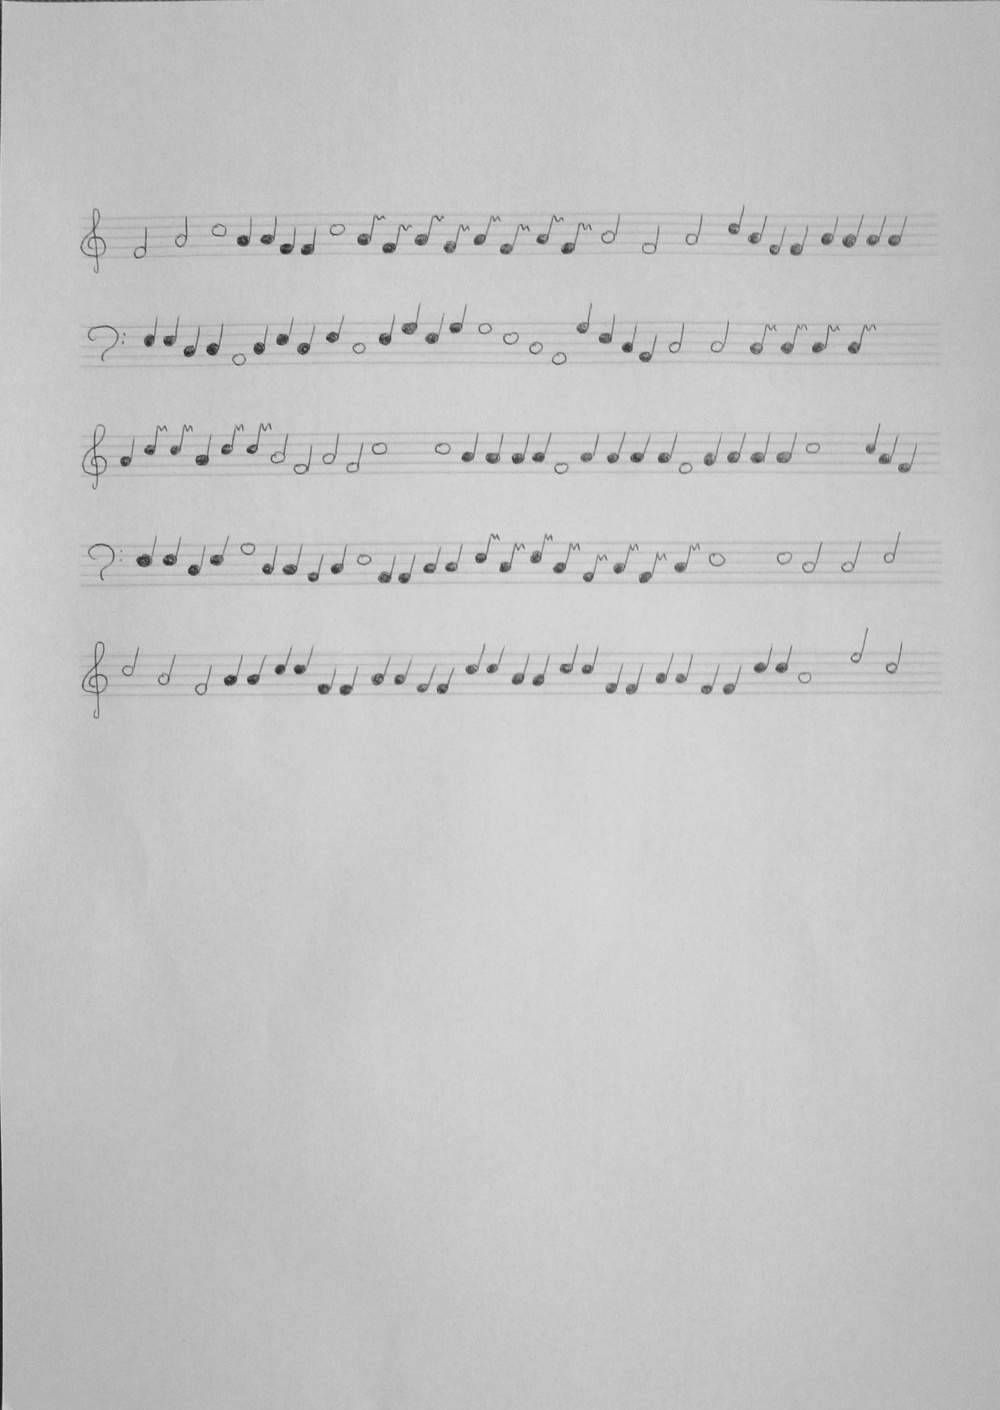
\includegraphics[width=.9\linewidth]{warped4_gray.jpg}
        % \caption{A subfigure}
        \label{fig:sub2}
    \end{subfigure}
    % \caption{Obraz oryginalny i po wycięciu}
    \label{fig:test}
\end{figure}
\begin{figure}
    \centering
    \begin{subfigure}{.5\textwidth}
        \centering
        \graphicspath{ {Resources/} }
        \includegraphics[width=.9\linewidth]{nutki_21.jpg}
        % \caption{A subfigure}
        \label{fig:sub1}
    \end{subfigure}%
    \begin{subfigure}{.5\textwidth}
        \centering
        \graphicspath{ {output/} }
        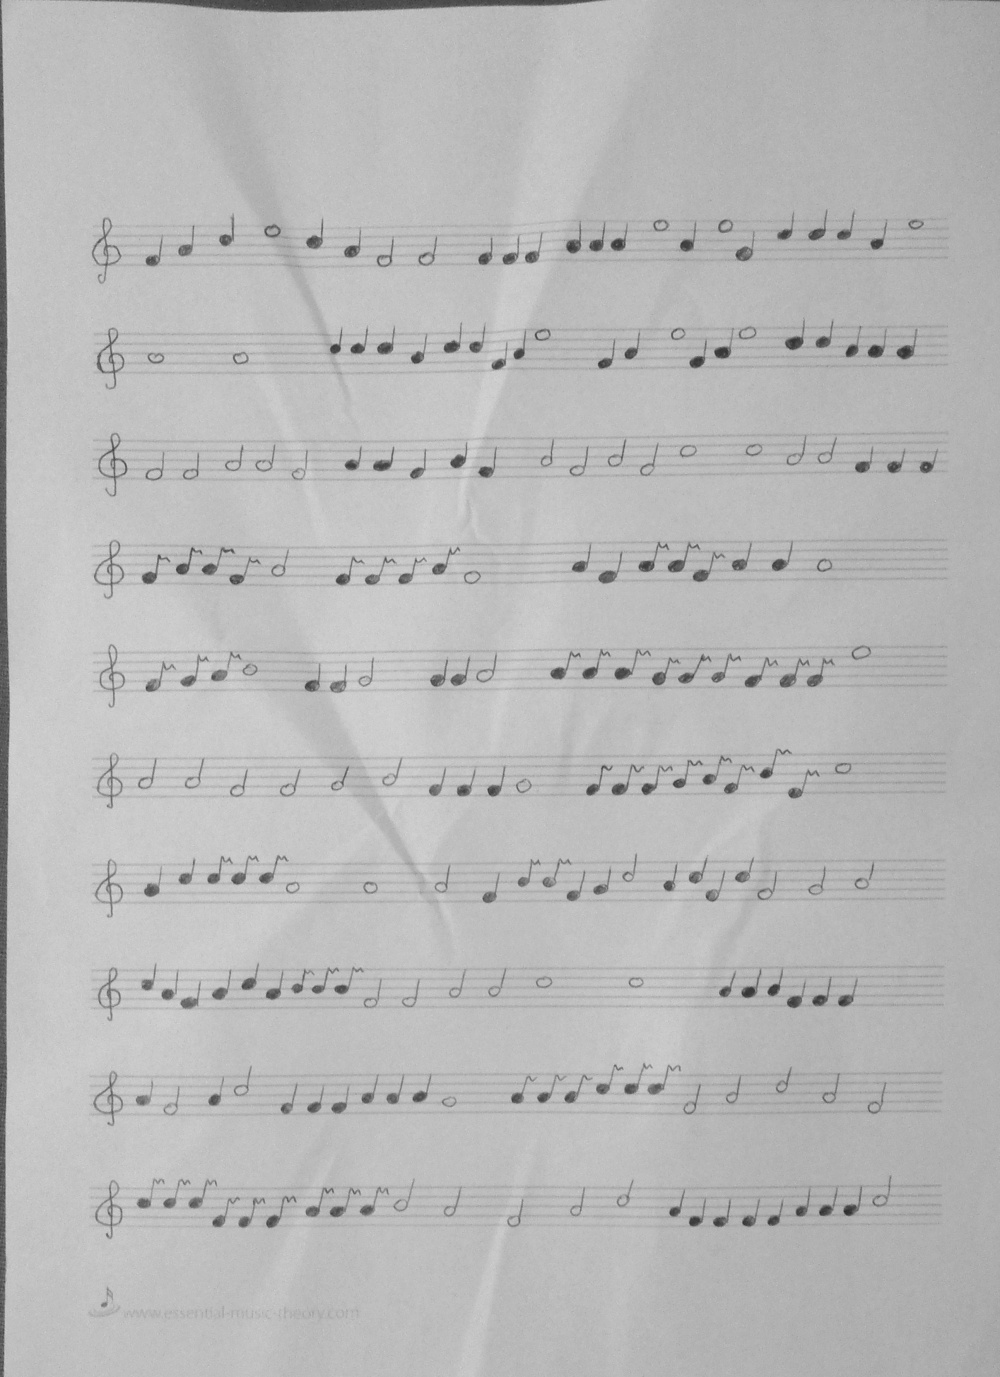
\includegraphics[width=.9\linewidth]{warped21_gray.jpg}
        % \caption{A subfigure}
        \label{fig:sub2}
    \end{subfigure}
    \caption{Obraz oryginalny i po wycięciu}
    \label{fig:test}
\end{figure}


\pagebreak

\begin{flushleft}
Nie dla wszystkich przypadków wykrywanie kartki zadziałało - dla nierównomiernego oświetlenia wykryte kontury kartki nie były zamknięte. 
Efekt takiego wycięcia wyglądał tak:
\end{flushleft}

\begin{figure}[h!]
\centering
\graphicspath{ {output/} }
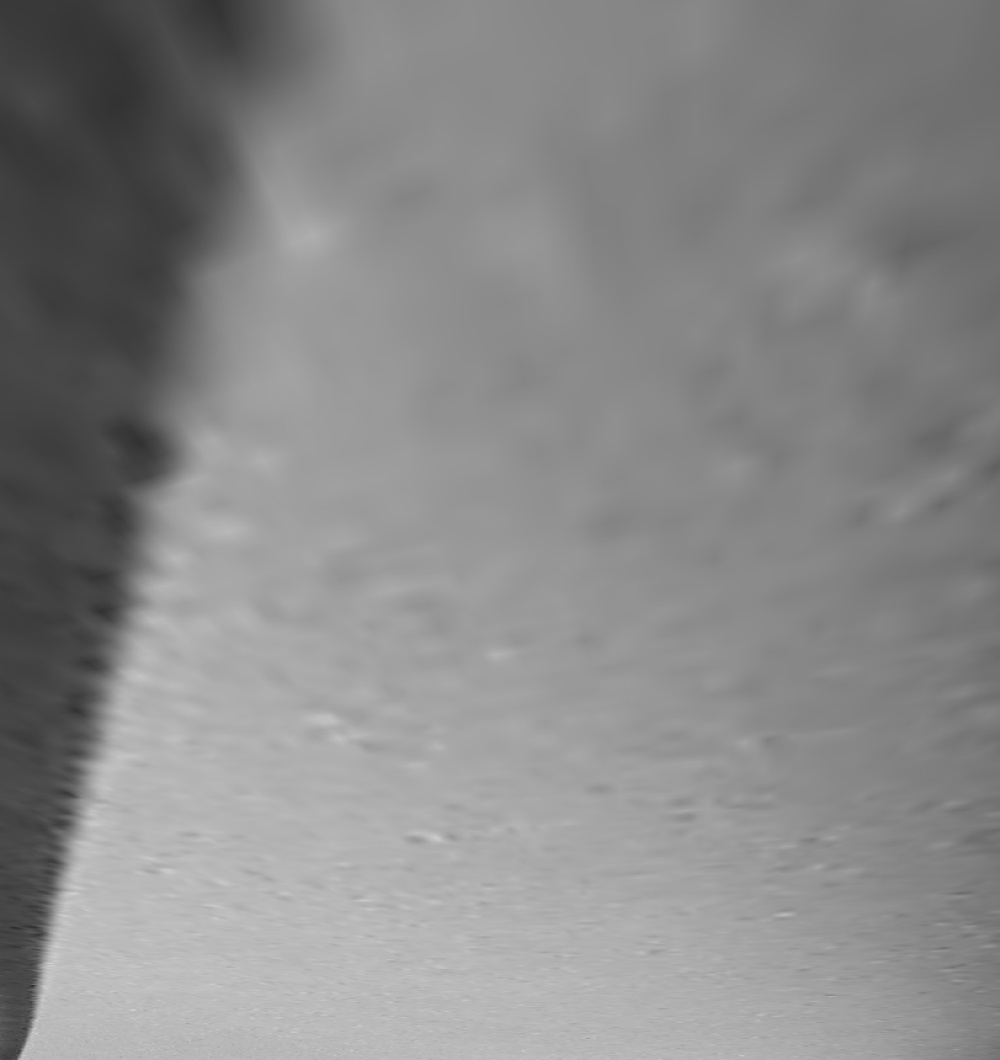
\includegraphics[scale=0.3]{warped15_gray.jpg}
\caption{Nieudany przykład}
\label{fig:universe}
\end{figure}

\pagebreak
\subsection{Wykrywanie pięciolinii}

Kolejnym zadaniem było wykrycie wysokości, na których znajdują się pięciolinie.
Zastosowaliśmy do tego transformacje Hougha do wykrywania linii. Skorzystaliśmy z gotowej funkcji \textbf{cv2.HoughLines}.
Jako jej parametry podaliśmy $\rho = 1 $ oraz $\theta = \pi / 100$ (ponieważ poszukujemy linii poziomych, kąt $\theta$ będzie niewielki, tak samo jak długość $\rho$).
Wcześniej jednak trzeba było przetworzyć obraz za pomocą funkcji threshold\_local oraz nakładając filtr Canny. 
Funkcja ta w zależności od jasności obrazu lepiej działała z parametrem 'method' ustawionym na 'median' albo 'mean'.
Zbyt duży threshold usuwał nutki, zbyt mały pozostawiał szumy i utrudniał wykrywanie nut.
Ostatecznie wybraliśmy nieco mniejszy i dodaliśmy erozję (cv2.erode()).
\newline

\begin{figure}[H]
    \centering
    \begin{subfigure}{.5\textwidth}
        \centering
        \graphicspath{ {staffs/} }
        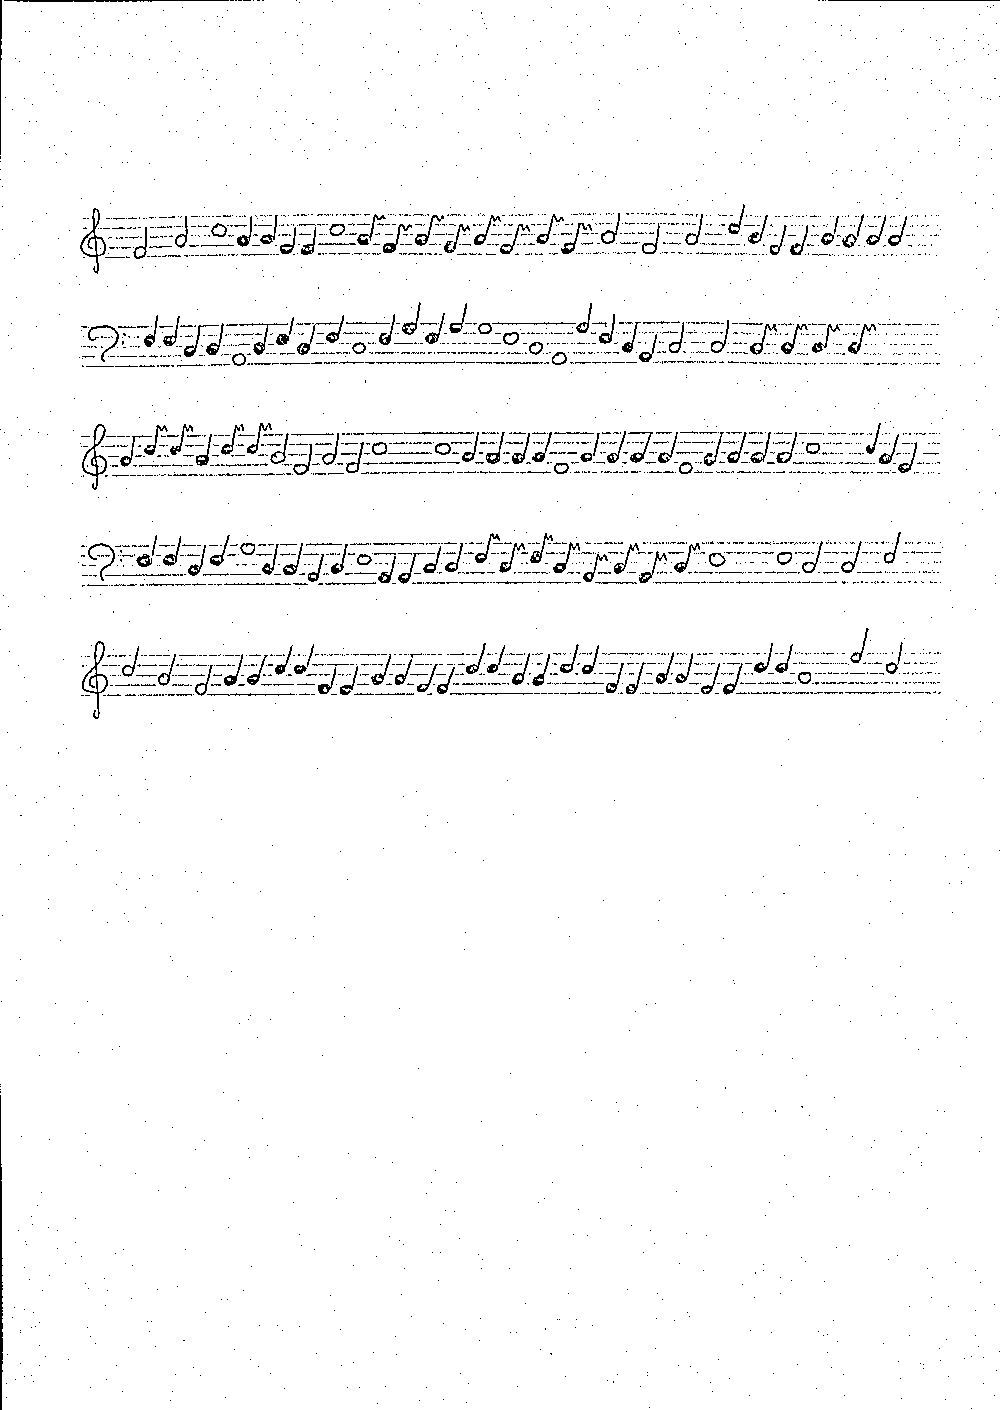
\includegraphics[width=\linewidth]{staffs4_thr.png}
        \caption{Threshold}
        \label{fig:sub1}
    \end{subfigure}%
    \begin{subfigure}{.5\textwidth}
        \centering
        \graphicspath{ {staffs/} }
        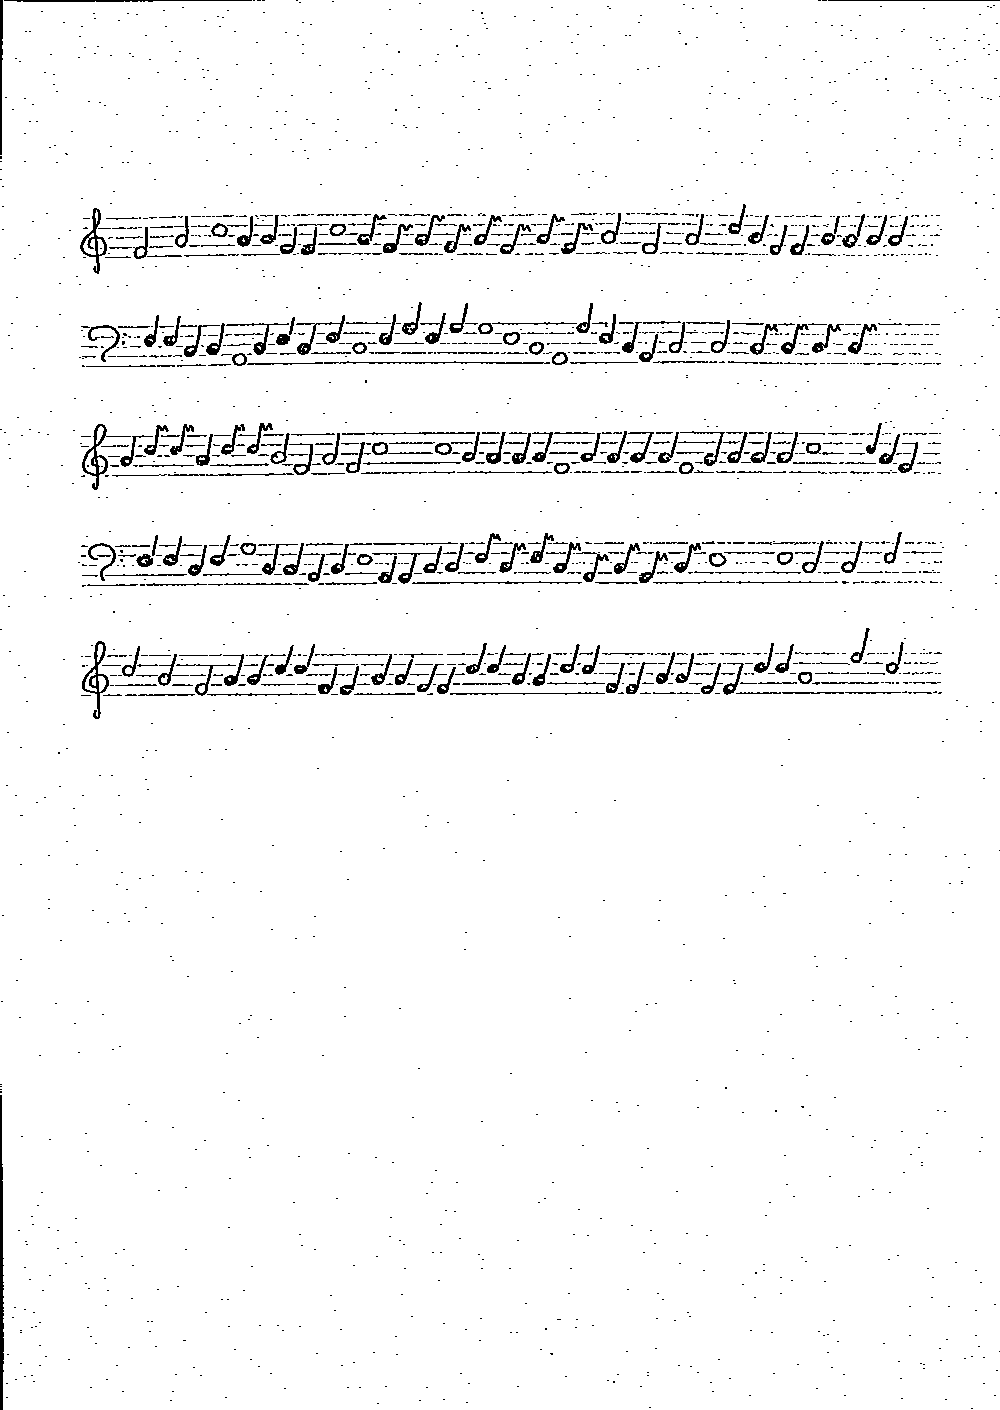
\includegraphics[width=\linewidth]{staffs4_erode.png}
        \caption{Erozja}
        \label{fig:sub2}
    \end{subfigure}
    % \caption{Obraz oryginalny i po wycięciu}
    \label{fig:test}
\end{figure}
\begin{figure}[H]
    \centering
    \begin{subfigure}{.5\textwidth}
        \centering
        \graphicspath{ {staffs/} }
        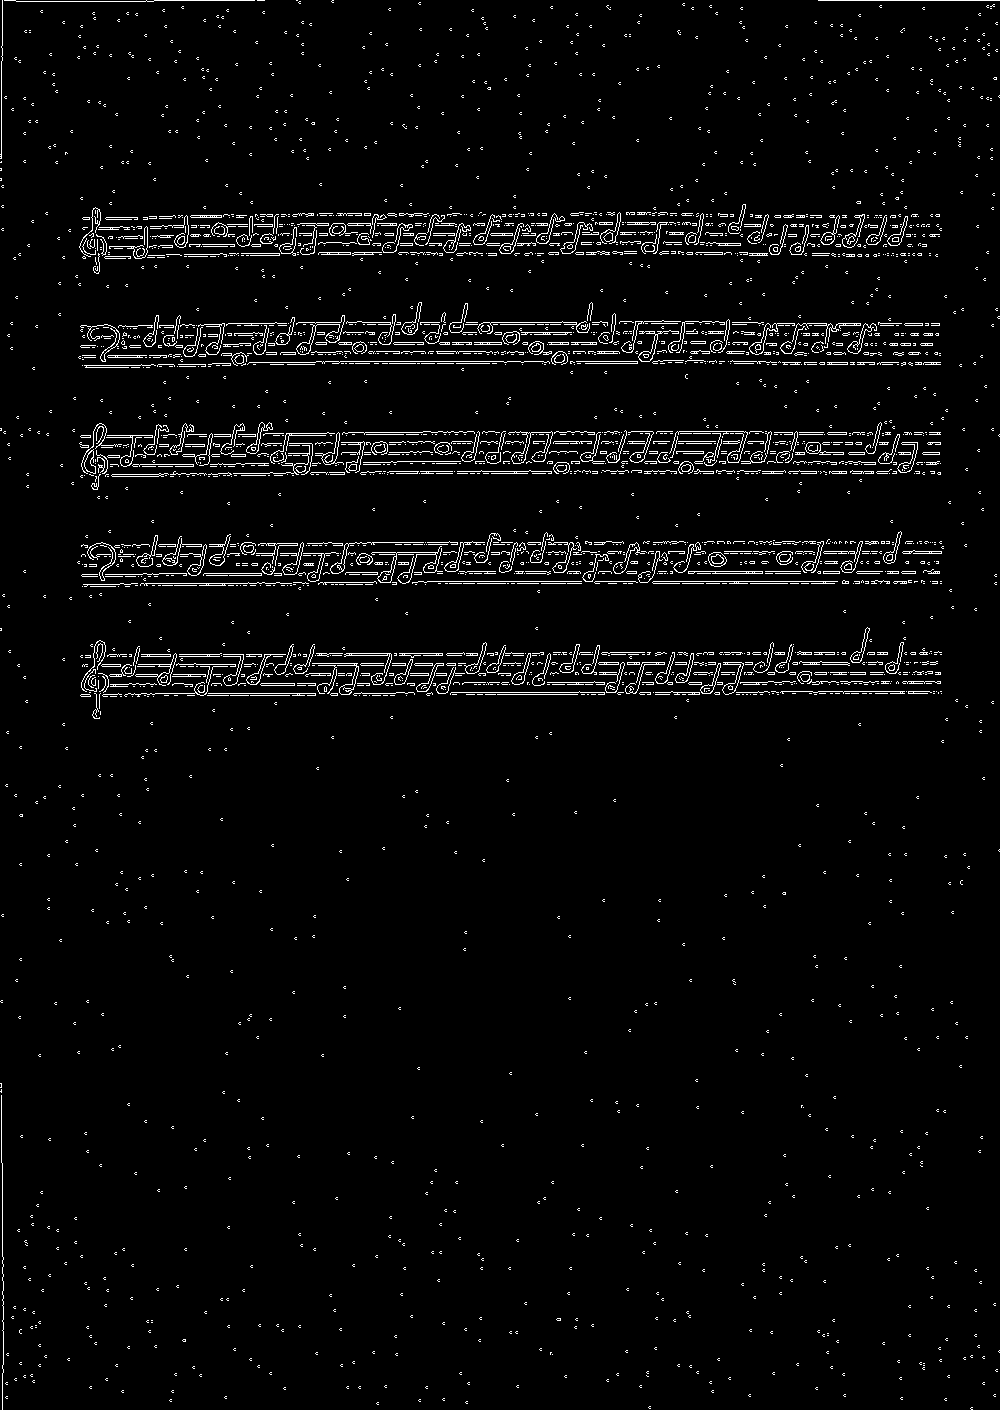
\includegraphics[width=.7\linewidth]{staffs4_canny.png}
        \caption{Canny}
        \label{fig:sub1}
    \end{subfigure}%
    \begin{subfigure}{.5\textwidth}
        \centering
        \graphicspath{ {staffs/} }
        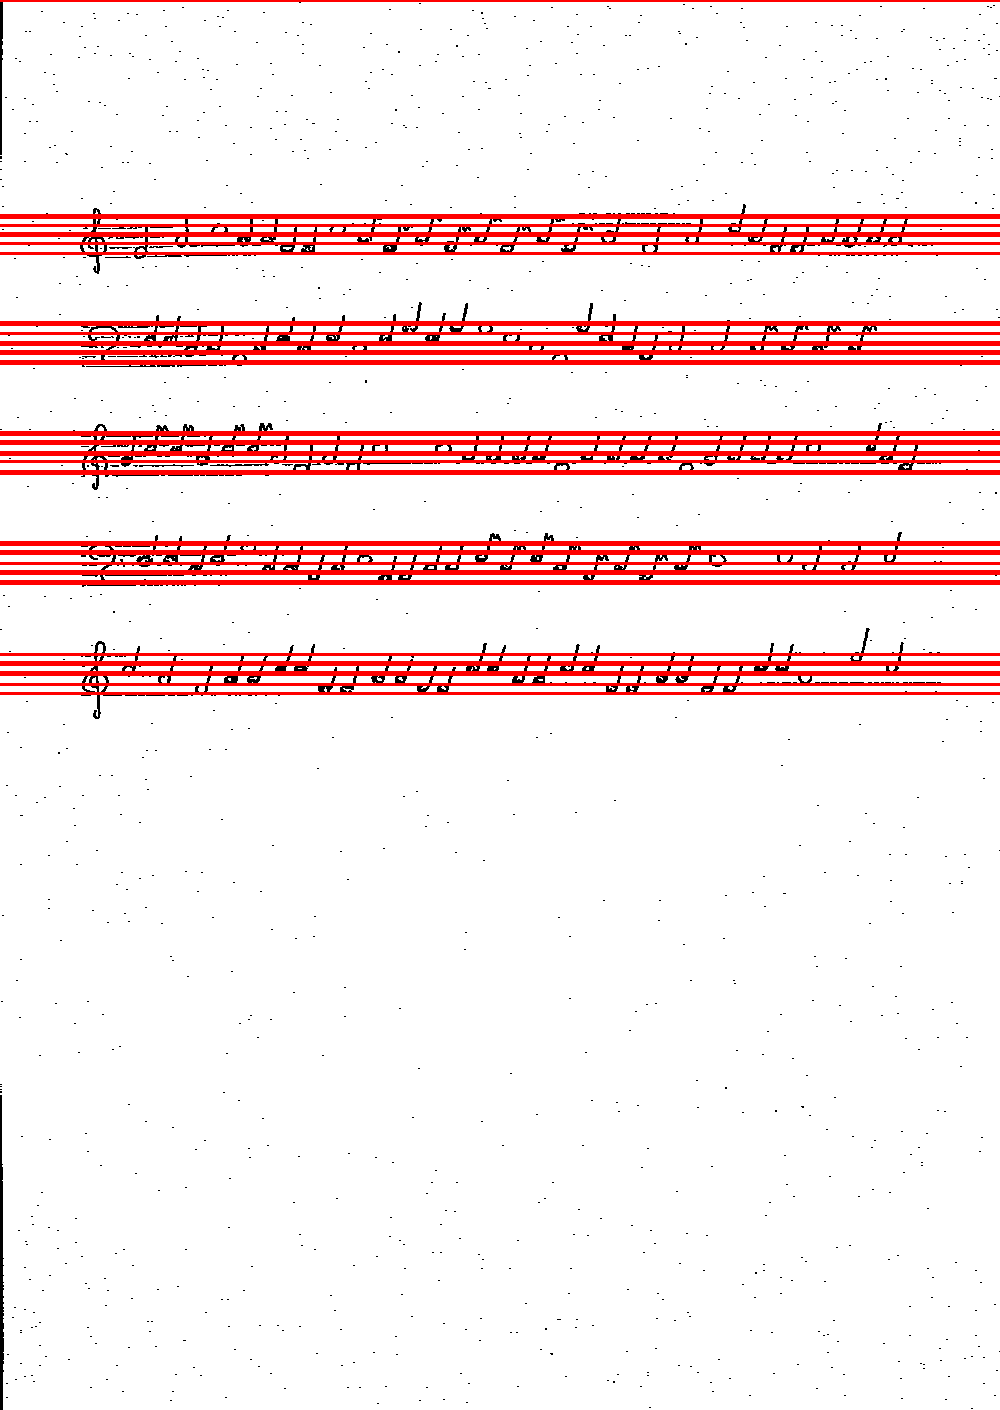
\includegraphics[width=.7\linewidth]{staffs4_lines.png}
        \caption{Wykryte linie}
        \label{fig:sub2}
    \end{subfigure}
    % \caption{Obraz oryginalny i po wycięciu}
    \label{fig:test}
\end{figure}

Po wykryciu linii za pomocą transformacji Hougha obliczamy współrzędne jej końców, a następnie centra.
Sprawdzając odległość pomiędzy liniami, stwierdzamy, czy należą one do jednej pięciolinii, czy też do dwóch różnych.
Jeśli znajdziemy pięć równoległych, leżących blisko siebie linii, zakładamy, że krańcowe z nich są granicami jednej z pięciolinii. 
Zwracamy obiekt Staff, który zawiera granice pięciolinii.

\begin{figure}[h!]
    \centering
    \graphicspath{ {staffs/} }
    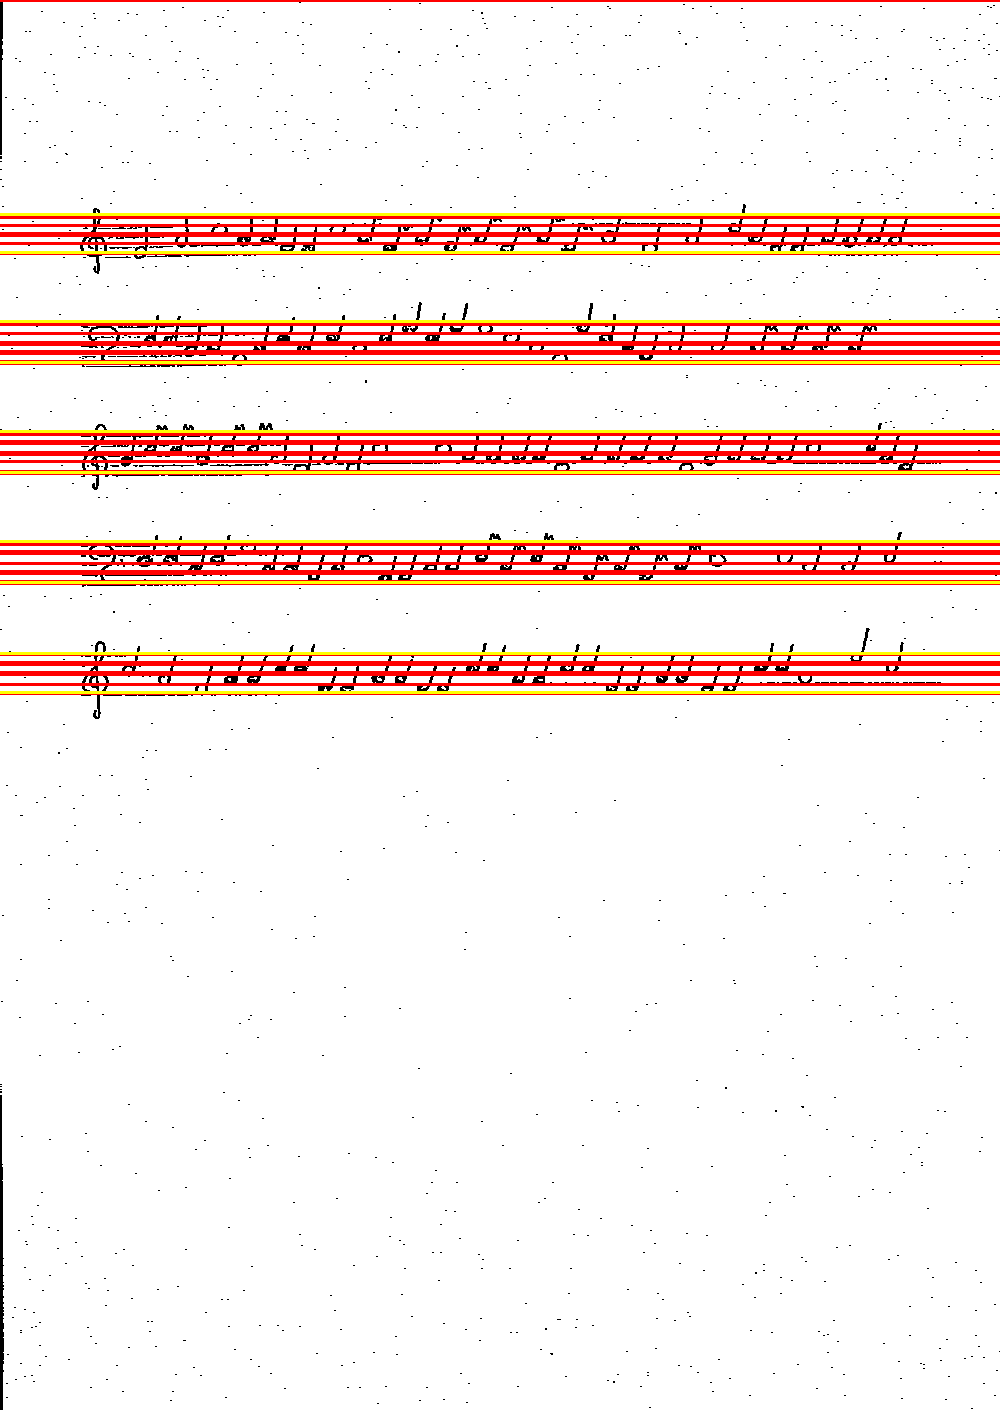
\includegraphics[scale=0.15]{staffs4_done.png}
    \caption{Wykryte pięciolinie}
    \label{fig:universe}
    \end{figure}

\subsection{Usuwanie pięciolinii}
Kolejnym krokiem jest usunięcie pięciolinii w celu łatwego wykrycia konturów nut.
W tym celu stosujemy na obrazie threshold, a następnie obracamy go w negatyw.
Do usunięcia pięciolinii używamy funkcji \newline
\textbf{cv2.getStructuringElement} oraz \textbf{cv2.morphologyEx}, 
z których pierwsza tworzy element, który będzie wyszukiwany i usuwany (w naszym przypadku będzie to długi cieńki prostokąt), 
a druga wykonuje wskazane przekształcenie morfologiczne (z parametrem \textbf{cv2.MORPH\_OPEN} wykonuje otwarcie - na zasadzie dylatacji)
Kolejnym krokiem jest wykonanie dość silnej erozji, aby struktura nut była pełna.
Następnie wyszukujemy kontury.
W przypadku wyszukiwania nut okrajamy nieco kartkę (przypisuję barwę białą pewnym marginesom),
aby uniknąć wyszukania tekstu na dole strony i kluczy wiolinowych/basowych.
Następnie kontury sortujemy po obwodach.
Wykrycie nut całych i ósemek jest trywialne (przedziały odpowiednio najmniejszych i największych obwodów).
W przypadku ćwierćnut i półnut, które mają ten sam rozmiar, sprawdzam średnią wartość fragmentu obrazu wydzielonego
przez kontur nuty (półnuta jest biała w środku - średnia wartość znacznie wyższa).
\newline

\begin{figure}[H]
    \centering
    \graphicspath{ {blobs/} }
    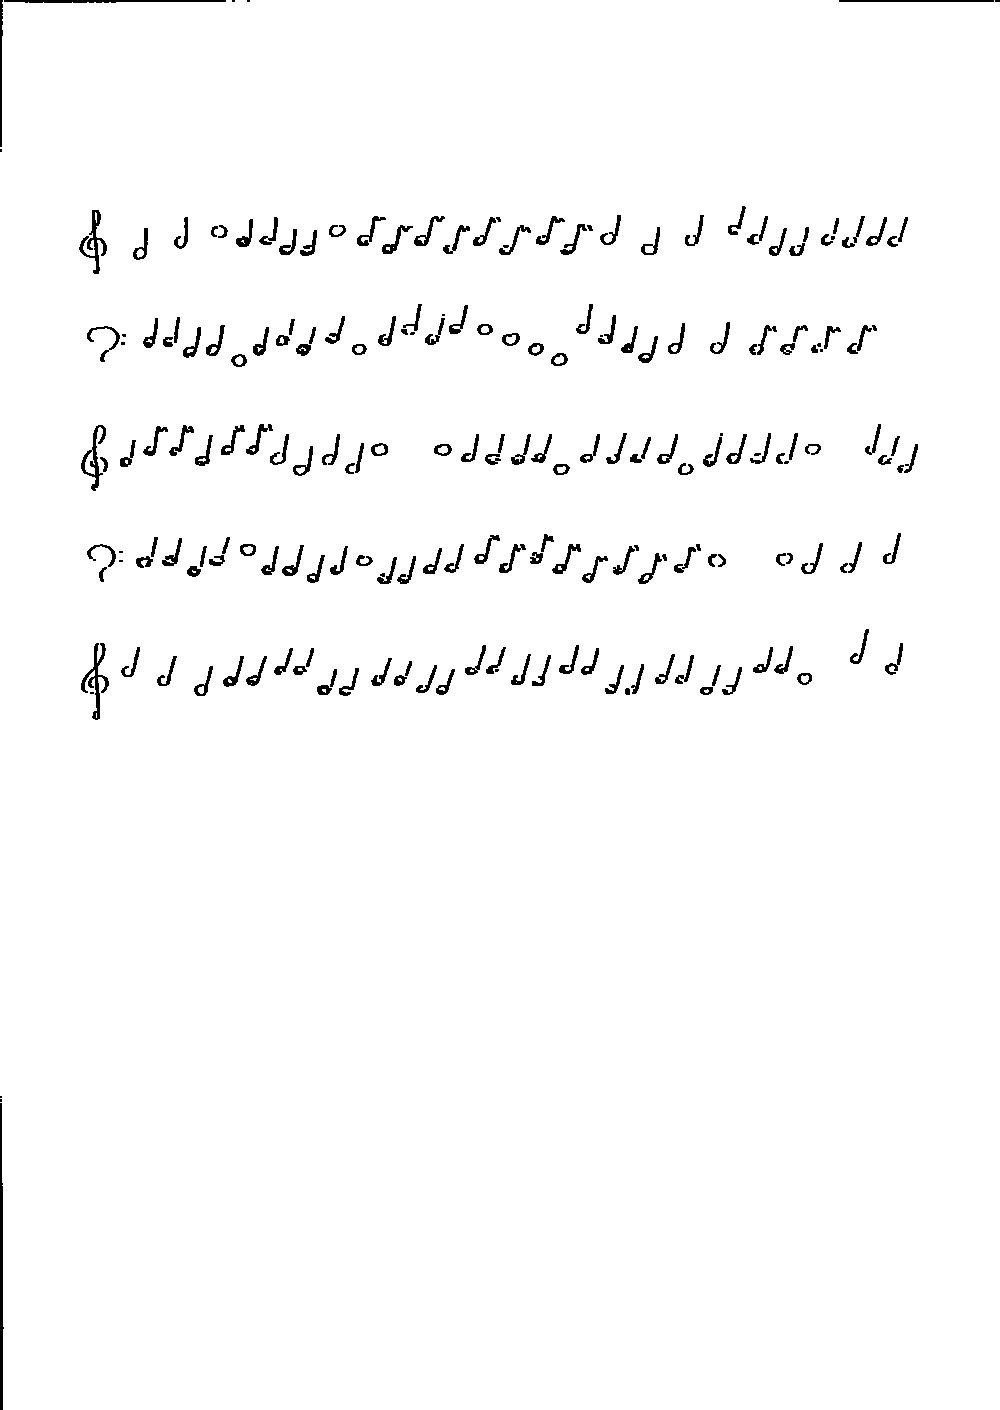
\includegraphics[scale=0.15]{4.jpg}
    \caption{Usunięte pięciolinie + silna erozja}
    \label{fig:universe}
    \end{figure}

\subsection{Wykrywanie kluczy}
Po skorzystaniu z utworzonych już funkcji do przekształcenia obrazu, znajdowania położenia każdej pięciolinii oraz usuwania ich z obraz pozostawiając możemy rozpocząć samo znajdowanie kluczy.
Przy szukaniu kluczy korzystamy z wiedzy, że muszą się one zawsze znajdować na początku pięciolinii. Wyznaczmy więc potencjalne miejsce klucza, proporcjonalnie do jego rozmiarów.
Następnie, korzystając z różnic pomiędzy kluczem wiolinowym, a kluczem basowym, będziemy przeszukiwać obszar pod pięciolinią. Szukamy pierwszego wystąpienia czarnego piksela. Jeśli jakiś się pojawił to znaczy że znaleźliśmy klucz wiolinowy, w przeciwnym wypadku znaleźliśmy klucz basowy.

\begin{figure}[H]
    \centering
    \begin{subfigure}{.5\textwidth}
        \centering
        \graphicspath{ {Resources/} }
        \includegraphics[width=.9\linewidth]{nutki_04.jpg}
        \label{figsub1}
    \end{subfigure}%
    \begin{subfigure}{.5\textwidth}
        \centering
        \graphicspath{ {keys/} }
        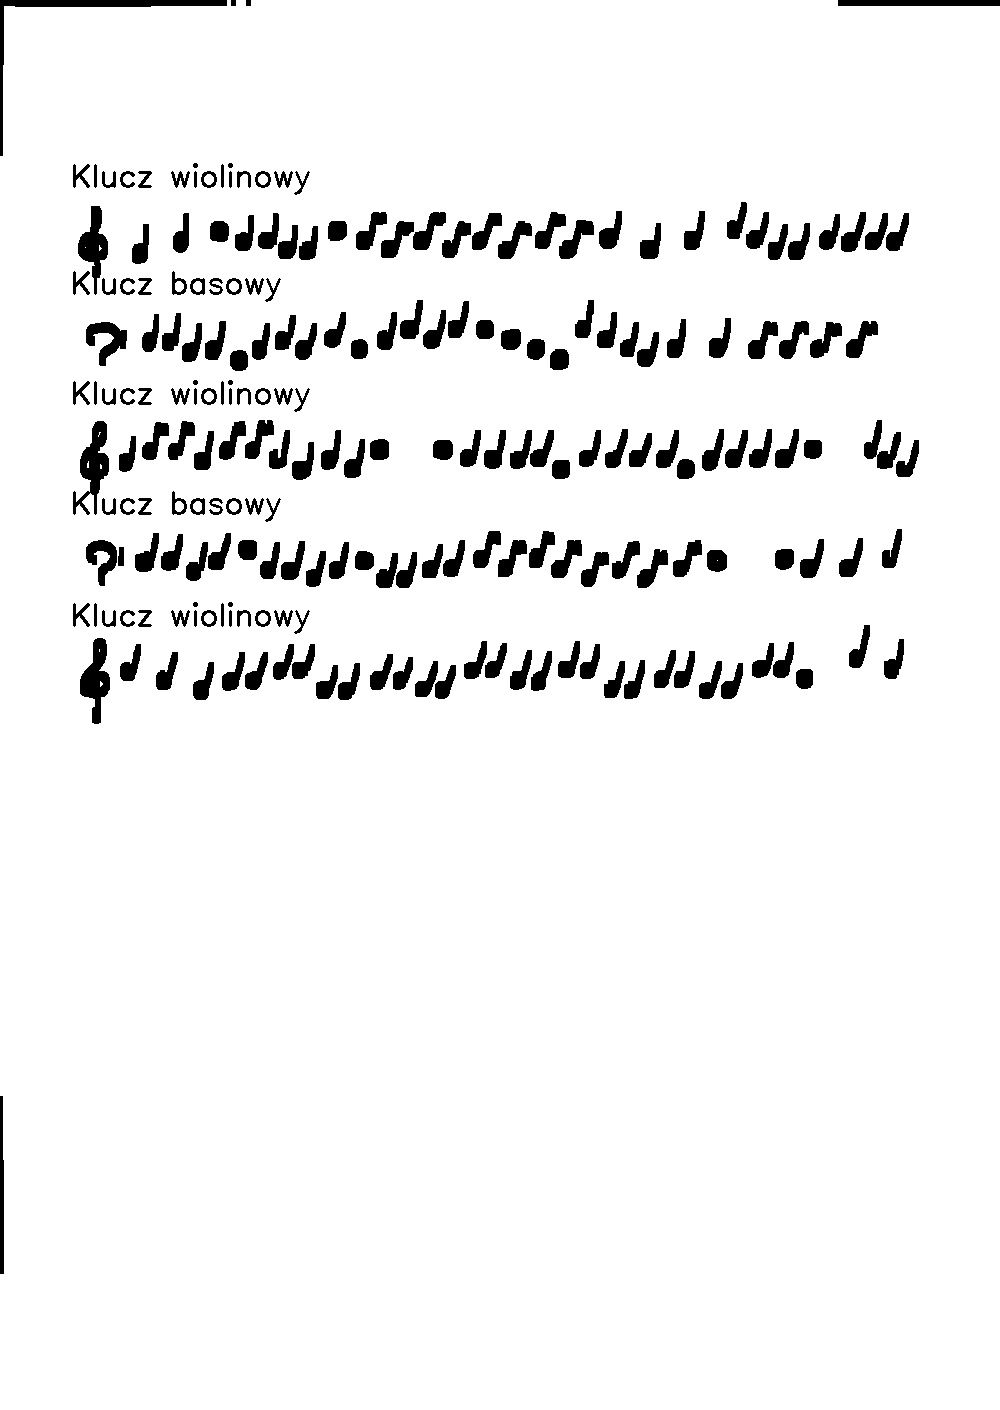
\includegraphics[width=.9\linewidth]{image_4.jpg}
        \label{figsub2}
    \end{subfigure}
    \label{figwykKlucze01}
\end{figure}
\begin{figure}[H]
    \centering
    \begin{subfigure}{.5\textwidth}
        \centering
        \graphicspath{ {Resources/} }
        \includegraphics[width=.9\linewidth]{nutki_21.jpg}
        \label{figsub1}
    \end{subfigure}%
    \begin{subfigure}{.5\textwidth}
        \centering
        \graphicspath{ {keys/} }
        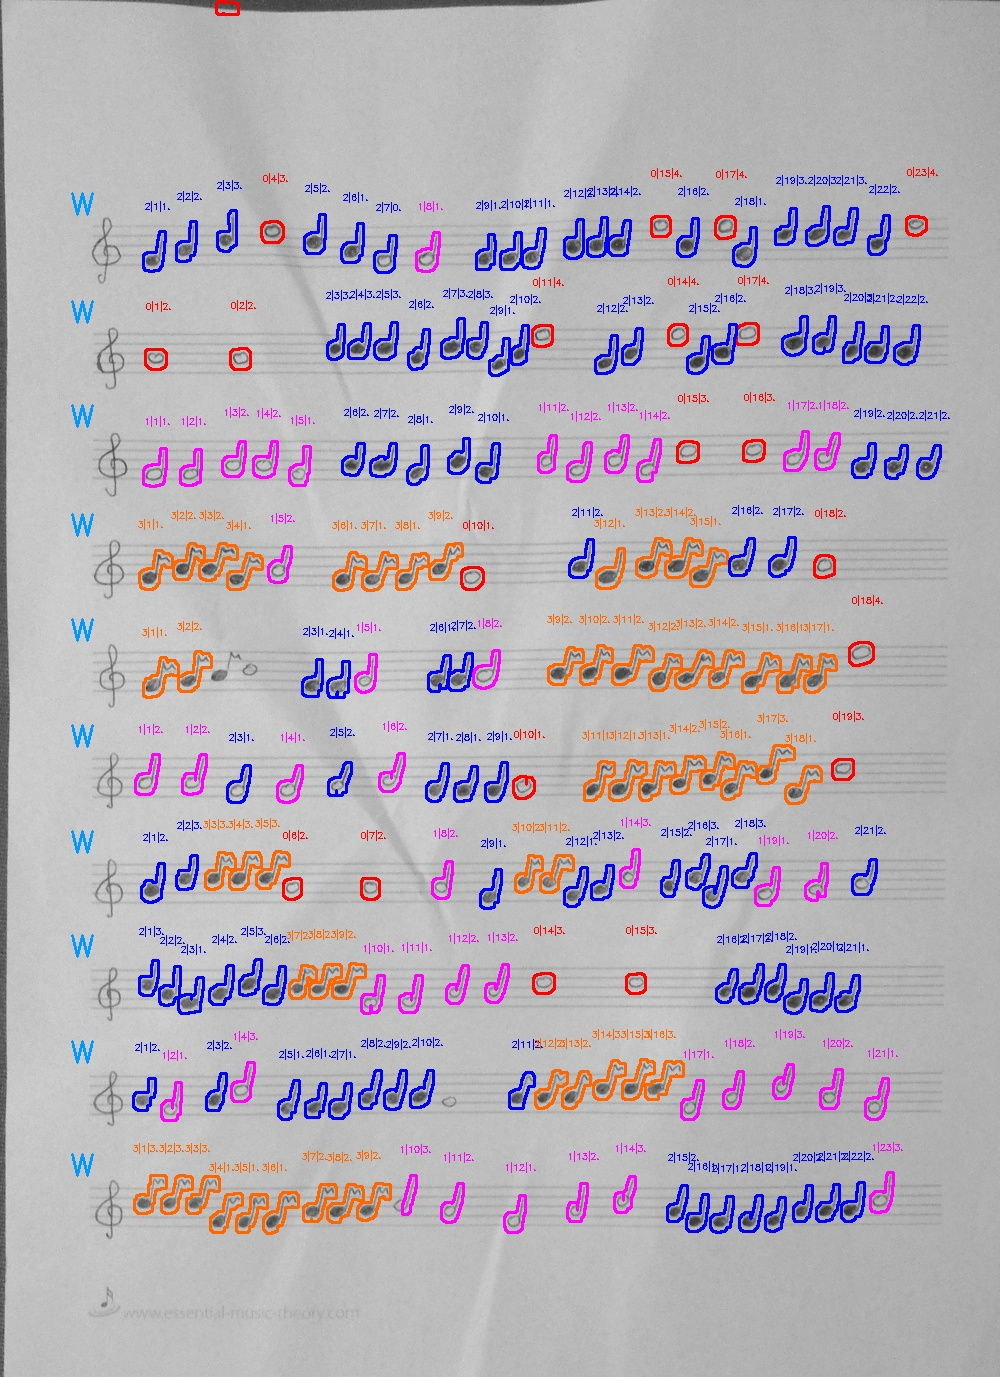
\includegraphics[width=.9\linewidth]{image_21.jpg}
        \label{figsub2}
    \end{subfigure}
    \caption{Obraz oryginalny i i ze znalezionymi kluczami}
    \label{figwygKlucze02}
\end{figure}

\subsection{TO DO}
Odpowiednie podpisywanie nut \newline
Połączenie wykrywania klucza z wykrywaniem nut\newline
Uszczególnienie parametrów podziału nut na całe/półnuty/ćwierćnuty/ósemki\newline


\section{Tymczasowe wyniki}

\subsection{Łatwe}

\begin{figure}[H]
    \centering
    \begin{subfigure}{.5\textwidth}
        \centering
        \graphicspath{ {Resources/} }
        \includegraphics[width=\linewidth]{nutki_04.jpg}
        % \caption{Threshold}
        \label{fig:sub1}
    \end{subfigure}%
    \begin{subfigure}{.5\textwidth}
        \centering
        \graphicspath{ {blobs/} }
        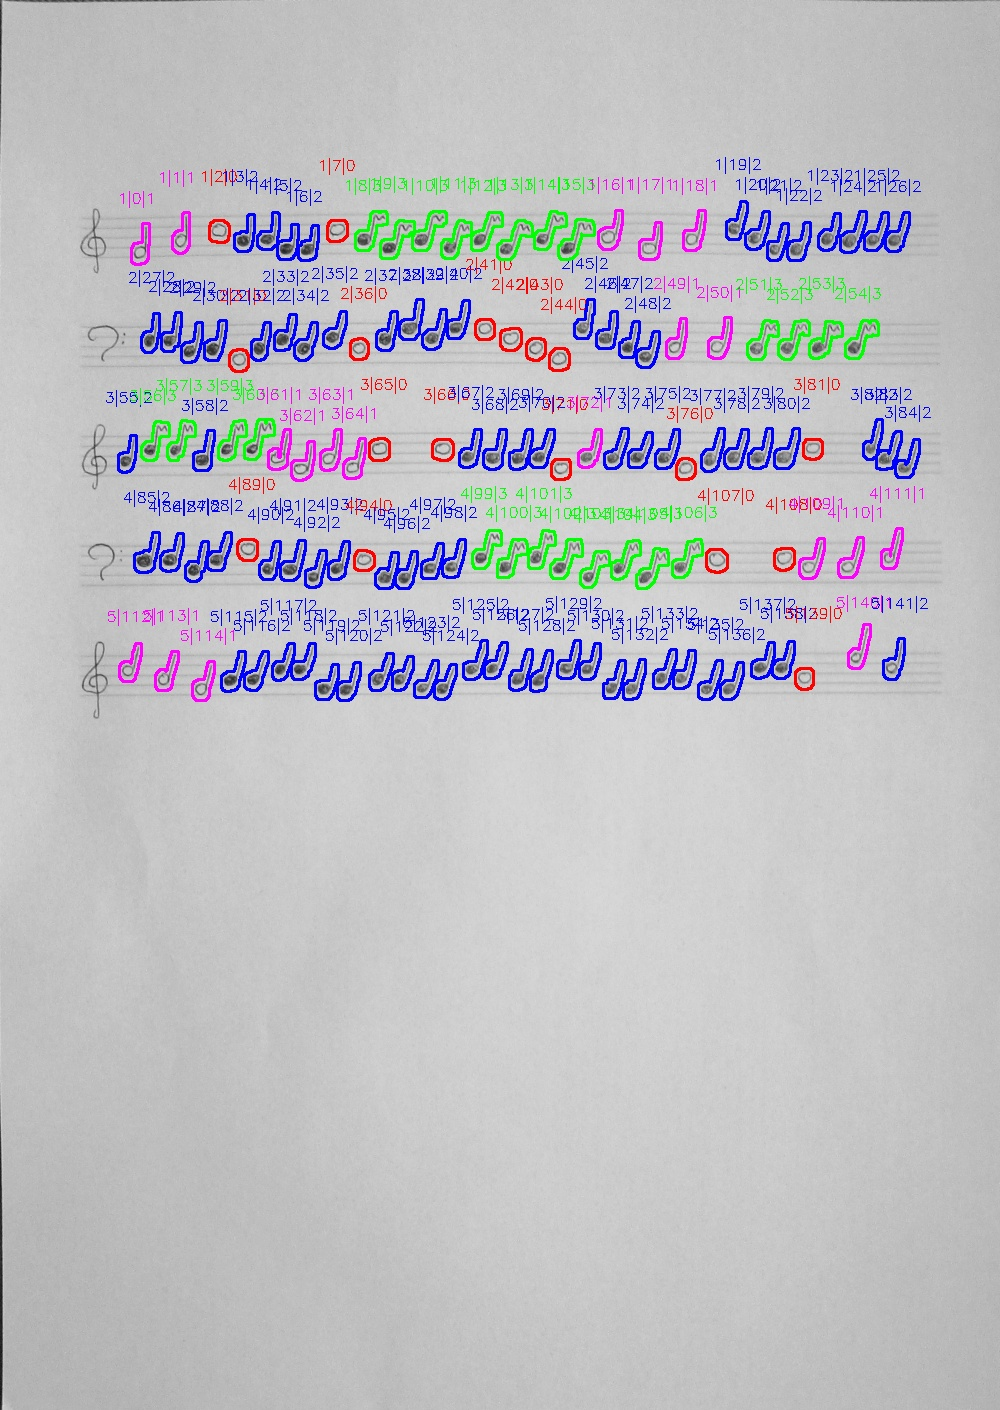
\includegraphics[width=\linewidth]{4_cnts.jpg}
        % \caption{Erozja}
        \label{fig:sub2}
    \end{subfigure}
    % \caption{Obraz oryginalny i po wycięciu}
    \label{fig:test}
\end{figure}

\begin{figure}[H]
    \centering
    \begin{subfigure}{.5\textwidth}
        \centering
        \graphicspath{ {Resources/} }
        \includegraphics[width=\linewidth]{nutki_05.jpg}
        % \caption{Threshold}
        \label{fig:sub1}
    \end{subfigure}%
    \begin{subfigure}{.5\textwidth}
        \centering
        \graphicspath{ {blobs/} }
        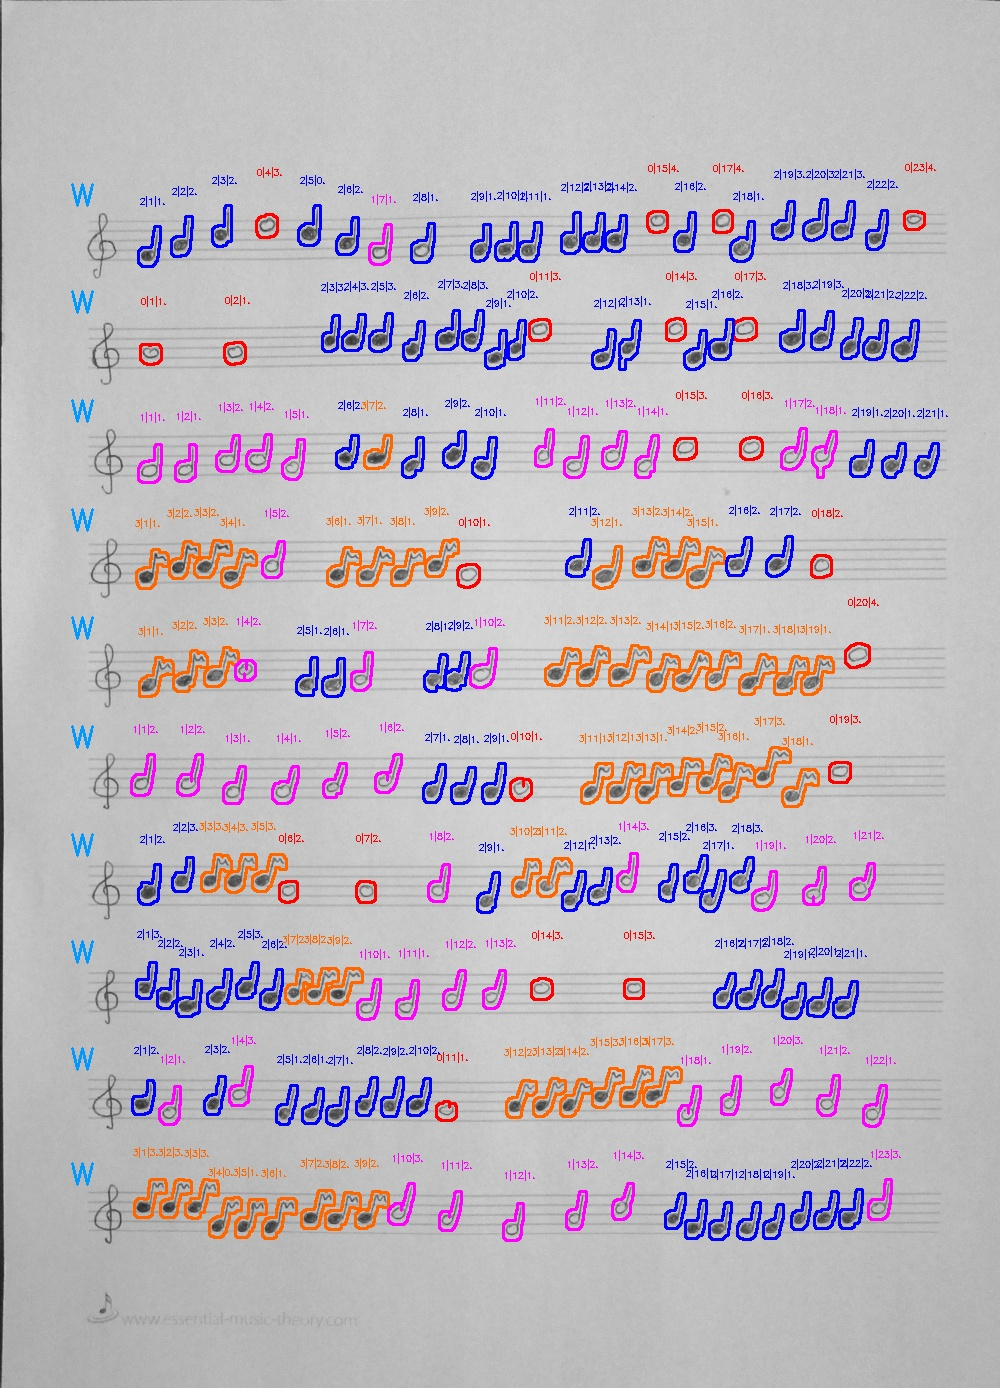
\includegraphics[width=\linewidth]{5_cnts.jpg}
        % \caption{Erozja}
        \label{fig:sub2}
    \end{subfigure}
    % \caption{Obraz oryginalny i po wycięciu}
    \label{fig:test}
\end{figure}

\begin{figure}[H]
    \centering
    \begin{subfigure}{.5\textwidth}
        \centering
        \graphicspath{ {Resources/} }
        \includegraphics[width=\linewidth]{nutki_06.jpg}
        % \caption{Threshold}
        \label{fig:sub1}
    \end{subfigure}%
    \begin{subfigure}{.5\textwidth}
        \centering
        \graphicspath{ {blobs/} }
        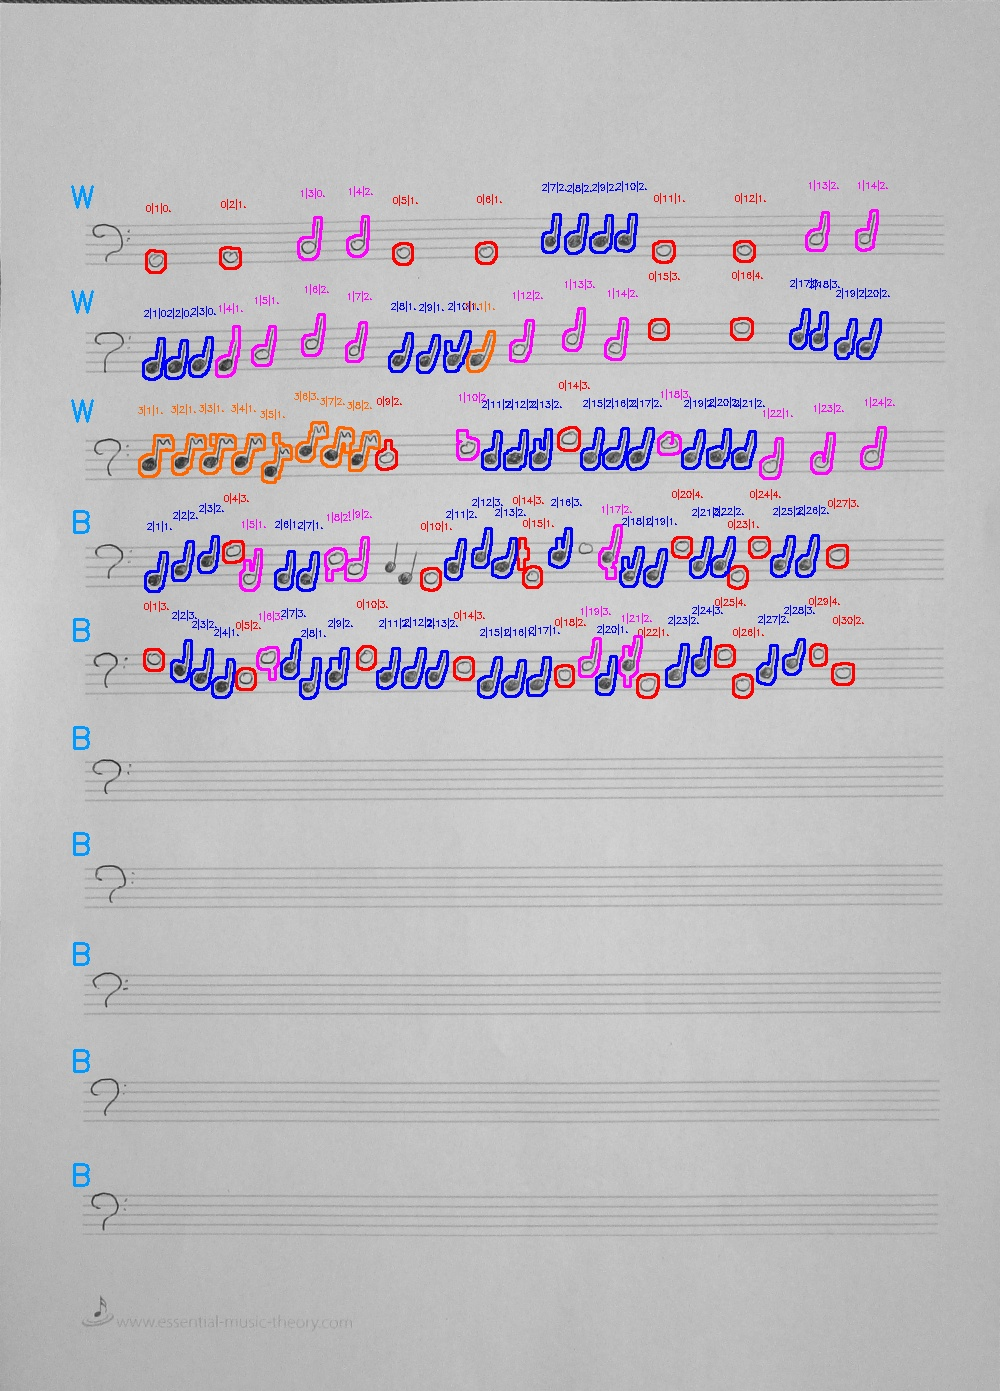
\includegraphics[width=\linewidth]{6_cnts.jpg}
        % \caption{Erozja}
        \label{fig:sub2}
    \end{subfigure}
    % \caption{Obraz oryginalny i po wycięciu}
    \label{fig:test}
\end{figure}

\begin{figure}[H]
    \centering
    \begin{subfigure}{.5\textwidth}
        \centering
        \graphicspath{ {Resources/} }
        \includegraphics[width=\linewidth]{nutki_08.jpg}
        % \caption{Threshold}
        \label{fig:sub1}
    \end{subfigure}%
    \begin{subfigure}{.5\textwidth}
        \centering
        \graphicspath{ {blobs/} }
        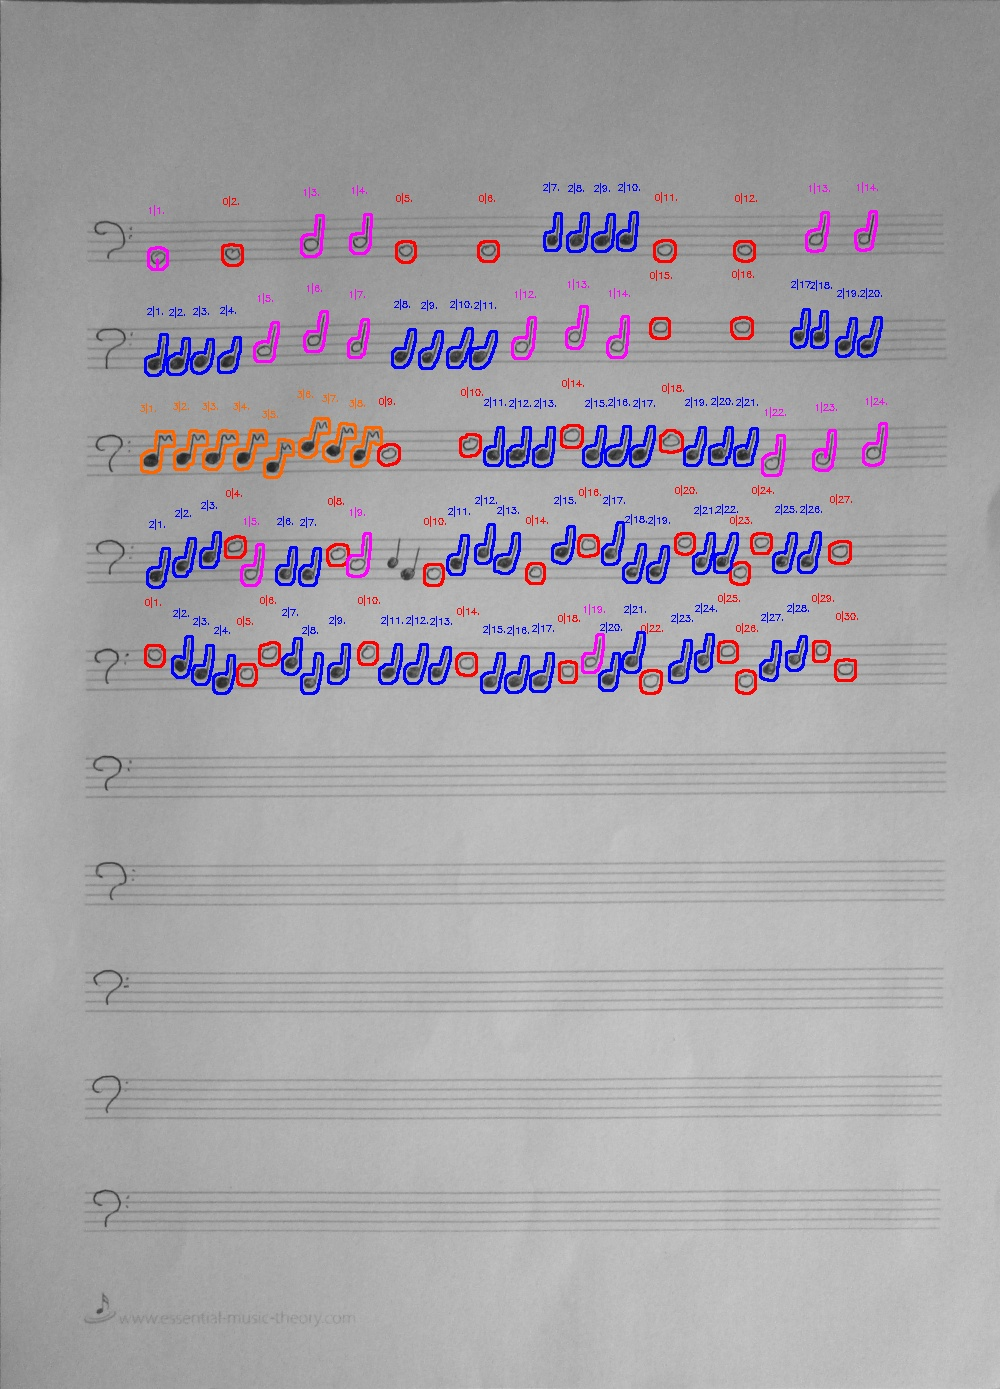
\includegraphics[width=\linewidth]{8_cnts.jpg}
        % \caption{Erozja}
        \label{fig:sub2}
    \end{subfigure}
    % \caption{Obraz oryginalny i po wycięciu}
    \label{fig:test}
\end{figure}

\begin{figure}[H]
    \centering
    \begin{subfigure}{.5\textwidth}
        \centering
        \graphicspath{ {Resources/} }
        \includegraphics[width=\linewidth]{nutki_13.jpg}
        % \caption{Threshold}
        \label{fig:sub1}
    \end{subfigure}%
    \begin{subfigure}{.5\textwidth}
        \centering
        \graphicspath{ {blobs/} }
        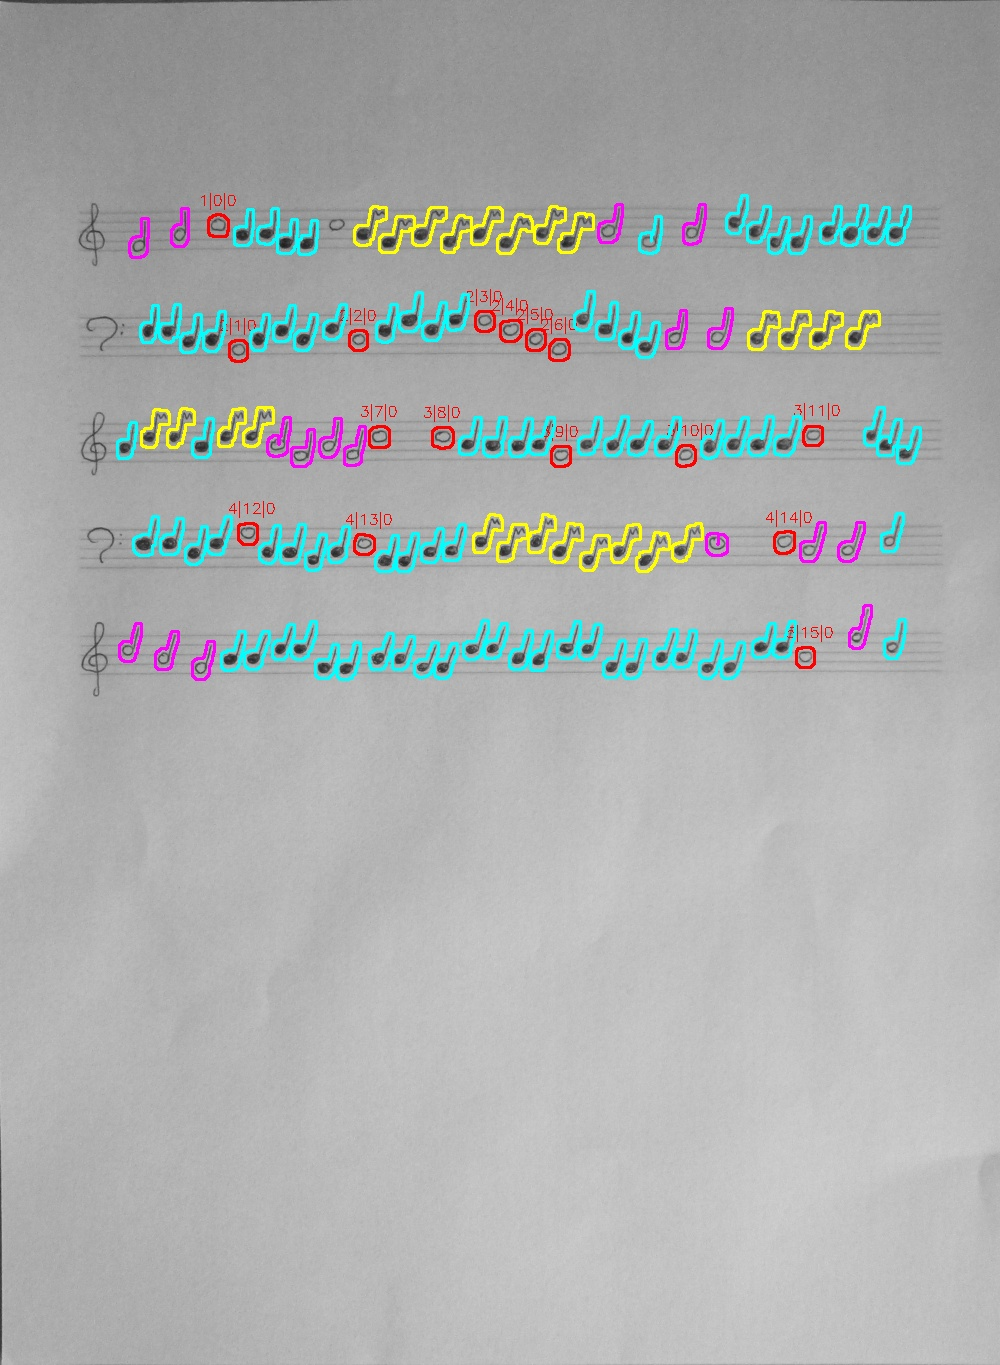
\includegraphics[width=\linewidth]{13_cnts.jpg}
        % \caption{Erozja}
        \label{fig:sub2}
    \end{subfigure}
    % \caption{Obraz oryginalny i po wycięciu}
    \label{fig:test}
\end{figure}

\subsection{Średnie}

\begin{figure}[H]
    \centering
    \begin{subfigure}{.5\textwidth}
        \centering
        \graphicspath{ {Resources/} }
        \includegraphics[width=\linewidth]{nutki_16.jpg}
        % \caption{Threshold}
        \label{fig:sub1}
    \end{subfigure}%
    \begin{subfigure}{.5\textwidth}
        \centering
        \graphicspath{ {blobs/} }
        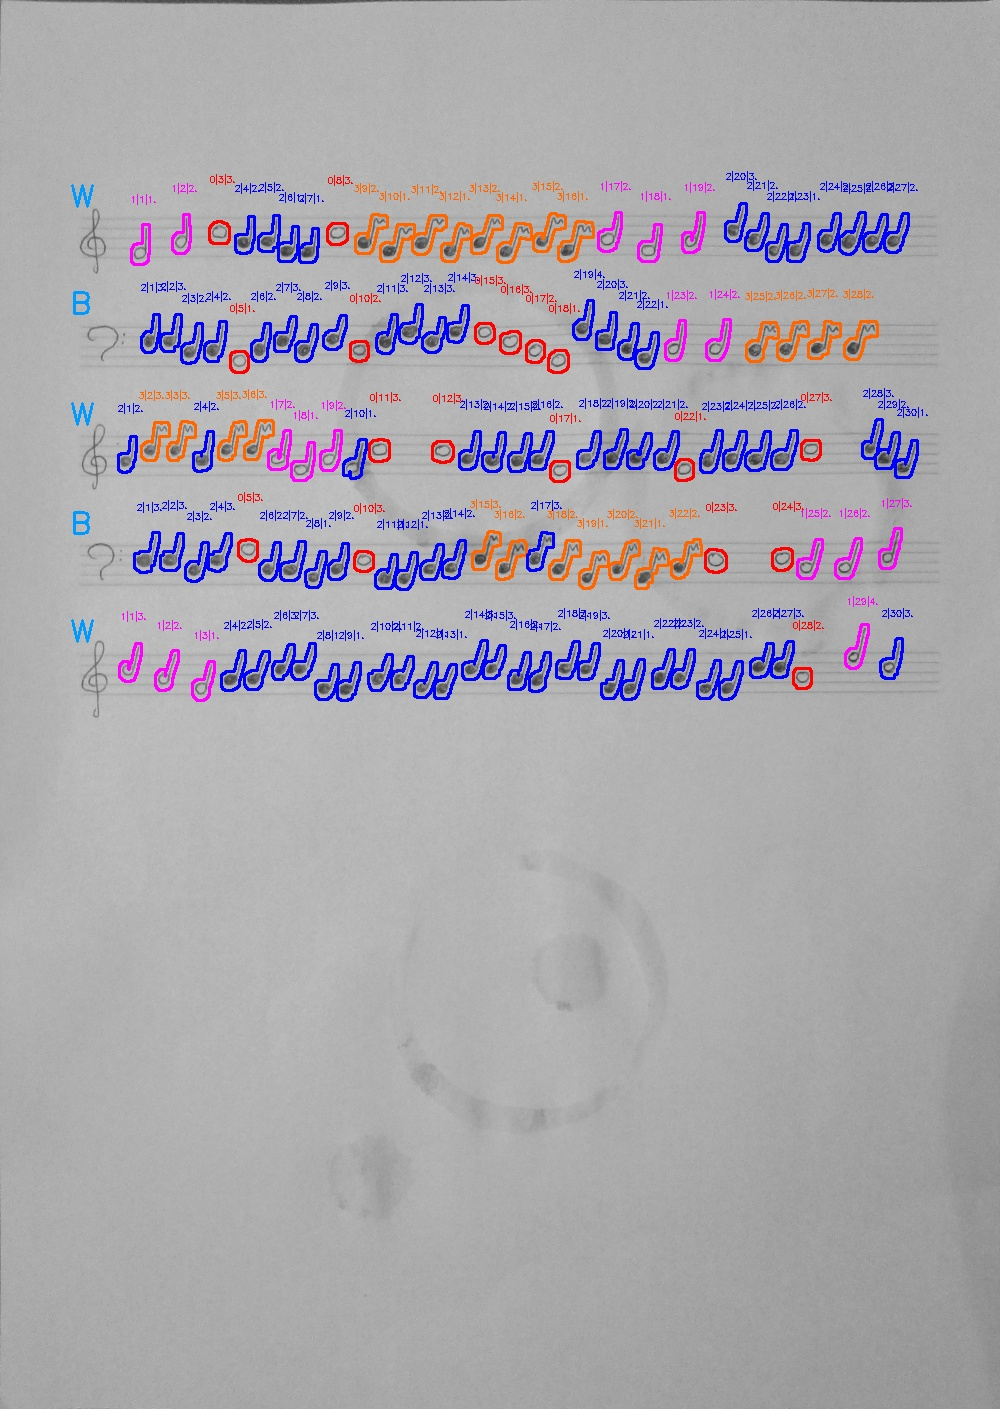
\includegraphics[width=\linewidth]{16_cnts.jpg}
        % \caption{Erozja}
        \label{fig:sub2}
    \end{subfigure}
    % \caption{Obraz oryginalny i po wycięciu}
    \label{fig:test}
\end{figure}

\begin{figure}[H]
    \centering
    \begin{subfigure}{.5\textwidth}
        \centering
        \graphicspath{ {Resources/} }
        \includegraphics[width=\linewidth]{nutki_17.jpg}
        % \caption{Threshold}
        \label{fig:sub1}
    \end{subfigure}%
    \begin{subfigure}{.5\textwidth}
        \centering
        \graphicspath{ {blobs/} }
        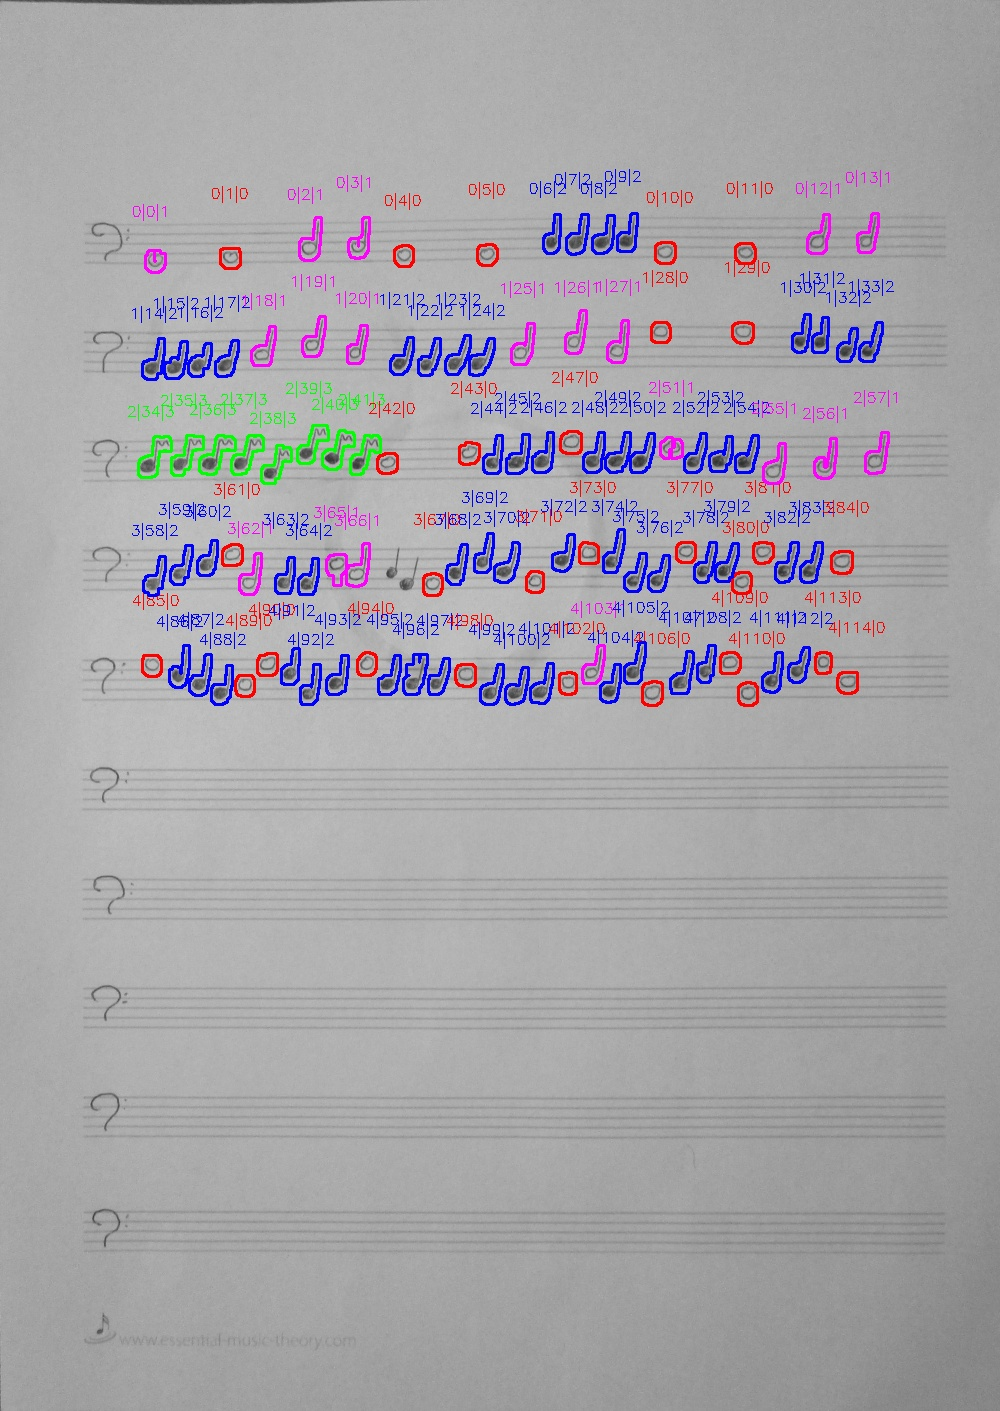
\includegraphics[width=\linewidth]{17_cnts.jpg}
        % \caption{Erozja}
        \label{fig:sub2}
    \end{subfigure}
    % \caption{Obraz oryginalny i po wycięciu}
    \label{fig:test}
\end{figure}

\begin{figure}[H]
    \centering
    \begin{subfigure}{.5\textwidth}
        \centering
        \graphicspath{ {Resources/} }
        \includegraphics[width=\linewidth]{nutki_20.jpg}
        % \caption{Threshold}
        \label{fig:sub1}
    \end{subfigure}%
    \begin{subfigure}{.5\textwidth}
        \centering
        \graphicspath{ {blobs/} }
        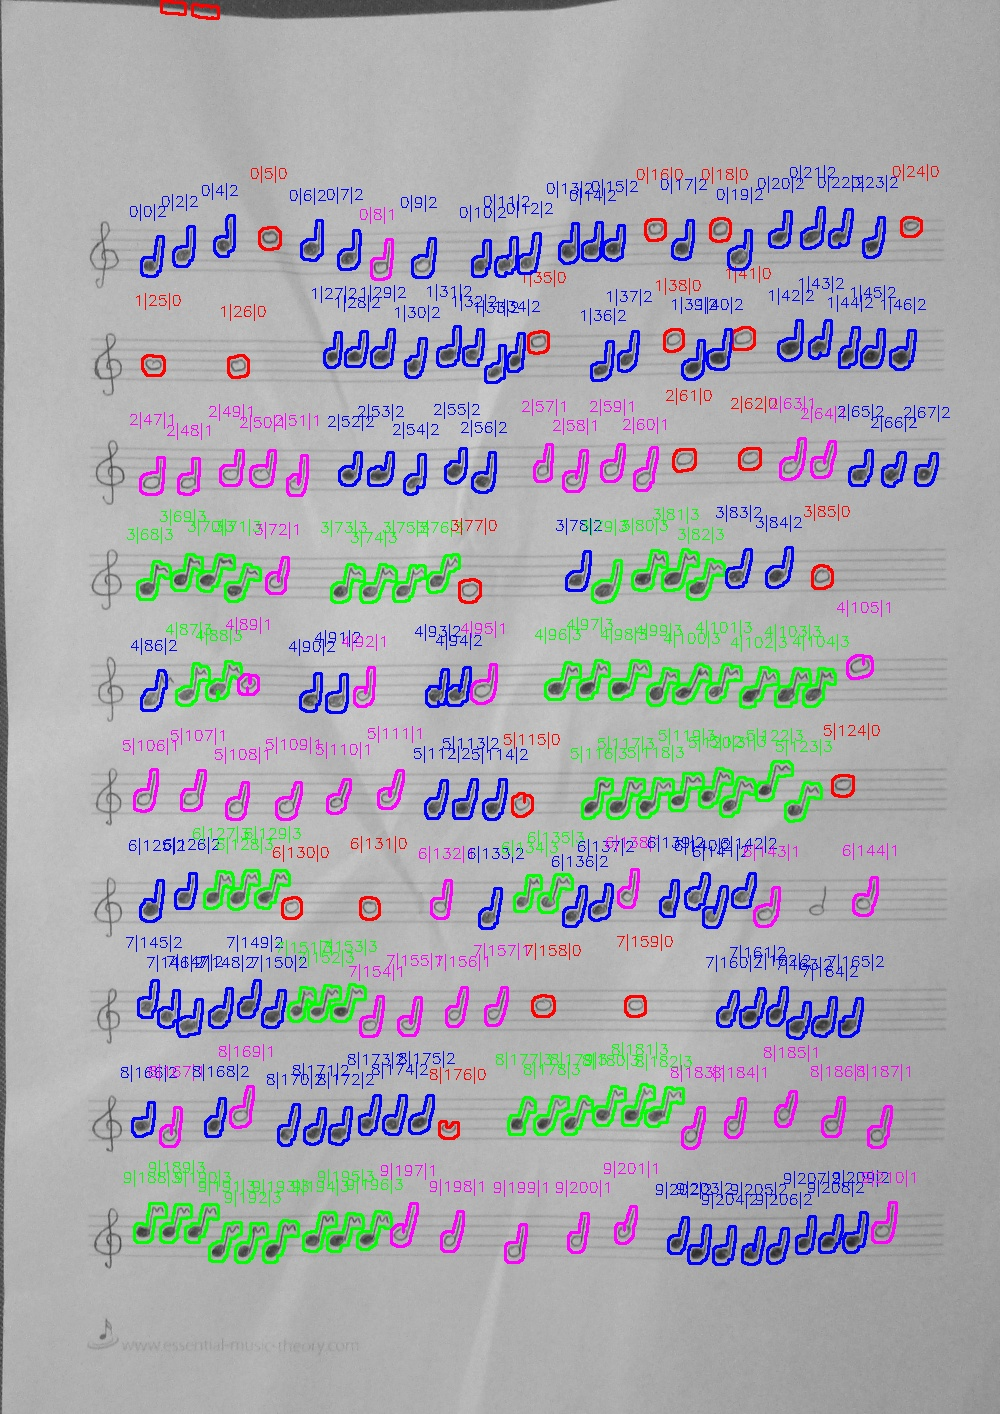
\includegraphics[width=\linewidth]{20_cnts.jpg}
        % \caption{Erozja}
        \label{fig:sub2}
    \end{subfigure}
    % \caption{Obraz oryginalny i po wycięciu}
    \label{fig:test}
\end{figure}

\begin{figure}[H]
    \centering
    \begin{subfigure}{.5\textwidth}
        \centering
        \graphicspath{ {Resources/} }
        \includegraphics[width=\linewidth]{nutki_21.jpg}
        % \caption{Threshold}
        \label{fig:sub1}
    \end{subfigure}%
    \begin{subfigure}{.5\textwidth}
        \centering
        \graphicspath{ {blobs/} }
        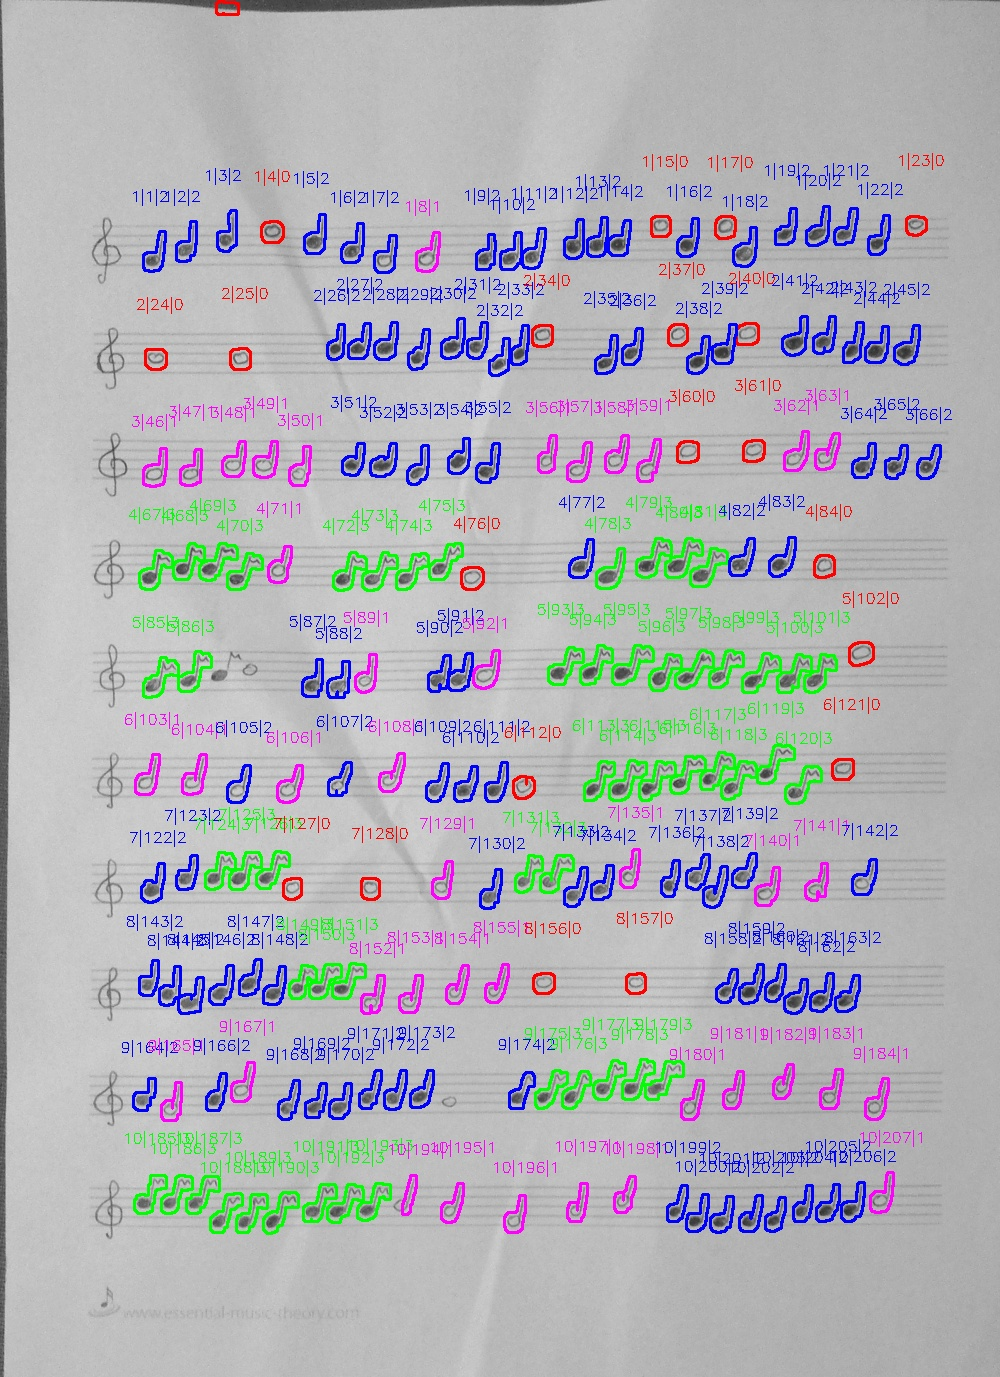
\includegraphics[width=\linewidth]{21_cnts.jpg}
        % \caption{Erozja}
        \label{fig:sub2}
    \end{subfigure}
    % \caption{Obraz oryginalny i po wycięciu}
    \label{fig:test}
\end{figure}

\begin{figure}[H]
    \centering
    \begin{subfigure}{.5\textwidth}
        \centering
        \graphicspath{ {Resources/} }
        \includegraphics[width=\linewidth]{nutki_41.jpg}
        % \caption{Threshold}
        \label{fig:sub1}
    \end{subfigure}%
    \begin{subfigure}{.5\textwidth}
        \centering
        \graphicspath{ {blobs/} }
        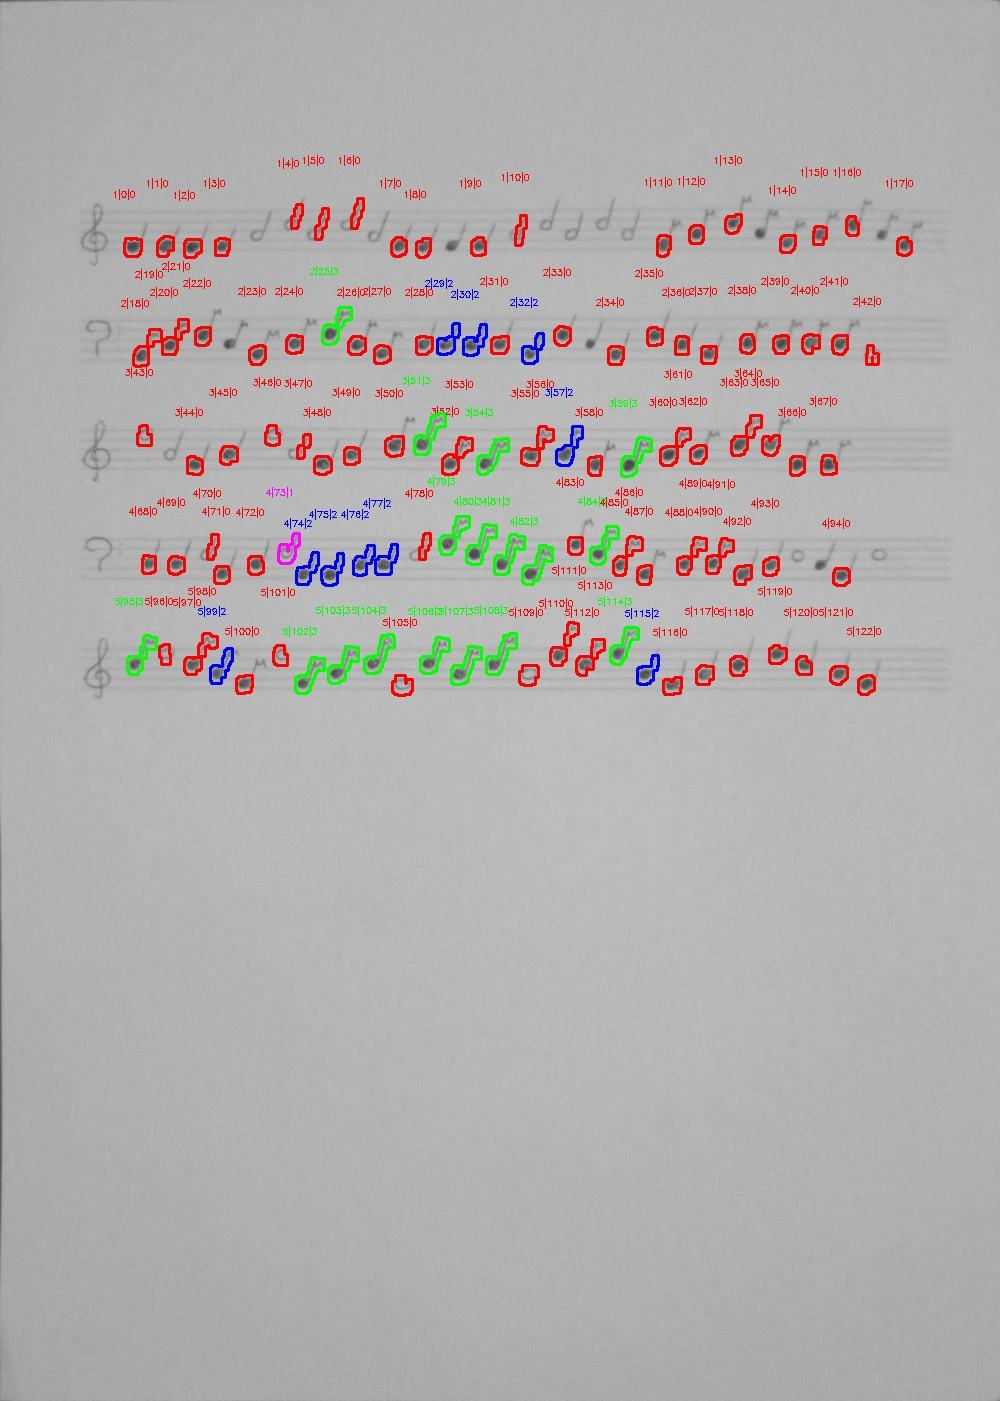
\includegraphics[width=\linewidth]{41_cnts.jpg}
        % \caption{Erozja}
        \label{fig:sub2}
    \end{subfigure}
    % \caption{Obraz oryginalny i po wycięciu}
    \label{fig:test}
\end{figure}



\subsection{Trudne}

\begin{figure}[H]
    \centering
    \begin{subfigure}{.5\textwidth}
        \centering
        \graphicspath{ {Resources/} }
        \includegraphics[width=\linewidth]{nutki_26.jpg}
        % \caption{Threshold}
        \label{fig:sub1}
    \end{subfigure}%
    \begin{subfigure}{.5\textwidth}
        \centering
        \graphicspath{ {blobs/} }
        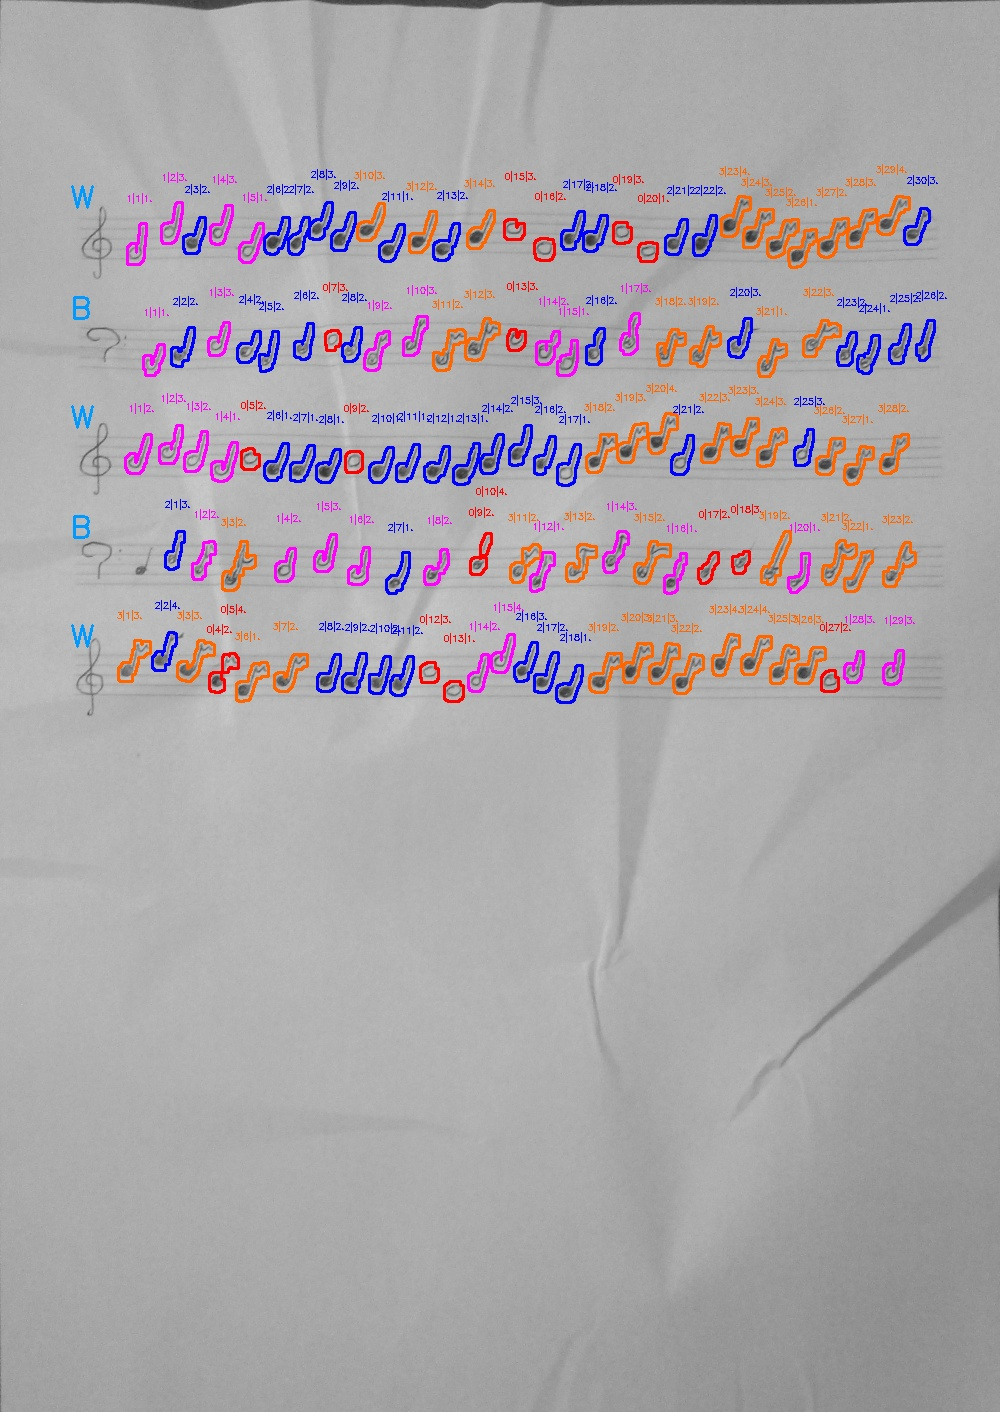
\includegraphics[width=\linewidth]{26_cnts.jpg}
        % \caption{Erozja}
        \label{fig:sub2}
    \end{subfigure}
    % \caption{Obraz oryginalny i po wycięciu}
    \label{fig:test}
\end{figure}

\begin{figure}[H]
    \centering
    \begin{subfigure}{.5\textwidth}
        \centering
        \graphicspath{ {Resources/} }
        \includegraphics[width=\linewidth]{nutki_27.jpg}
        % \caption{Threshold}
        \label{fig:sub1}
    \end{subfigure}%
    \begin{subfigure}{.5\textwidth}
        \centering
        \graphicspath{ {blobs/} }
        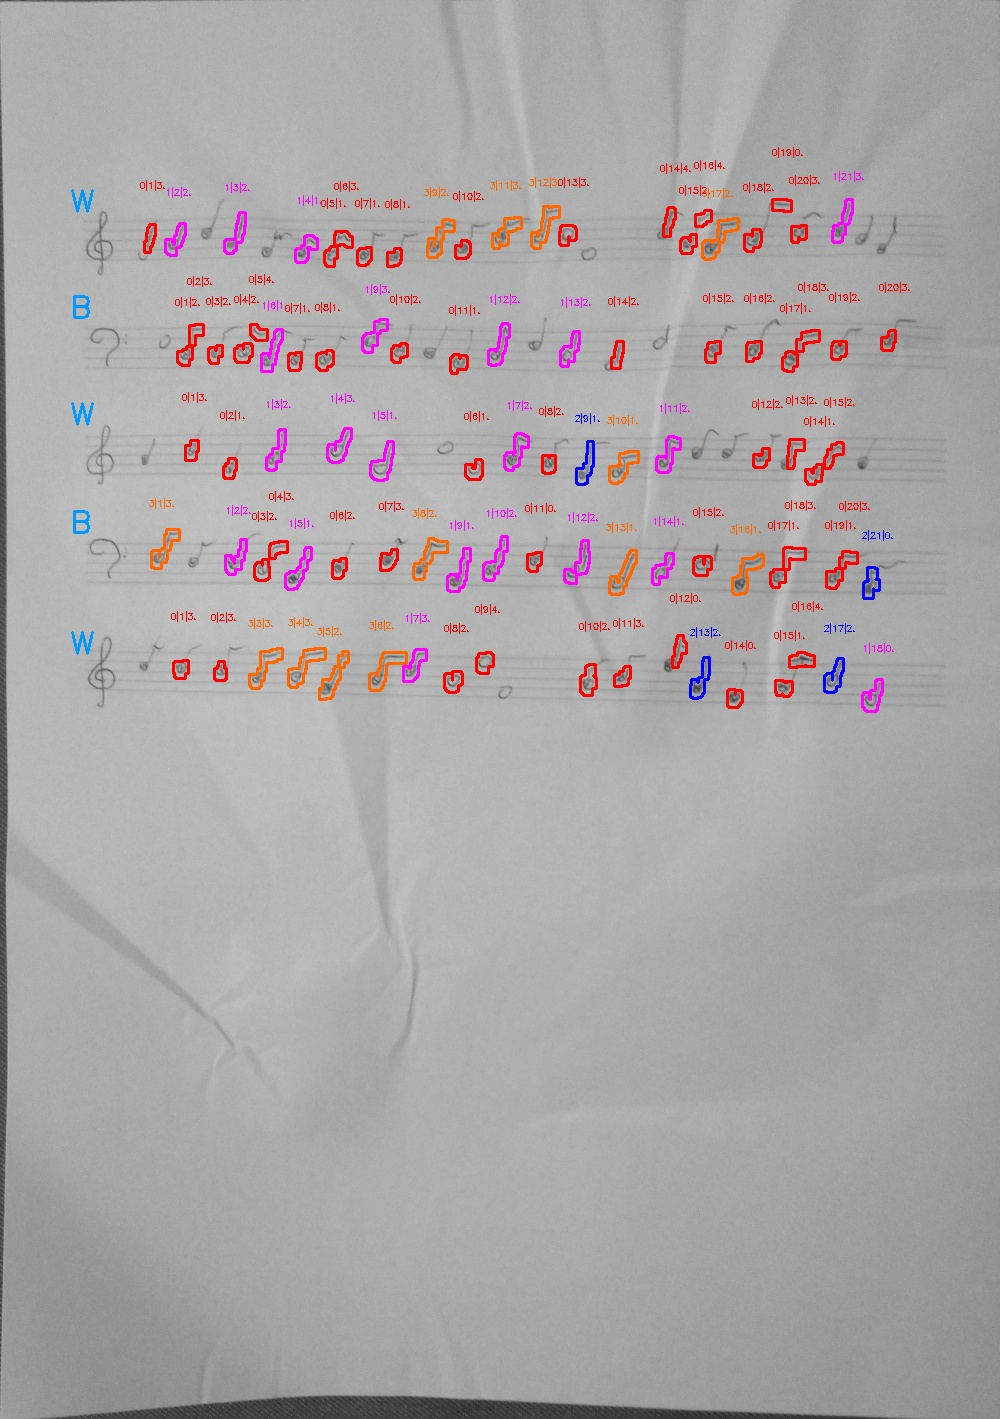
\includegraphics[width=\linewidth]{27_cnts.jpg}
        % \caption{Erozja}
        \label{fig:sub2}
    \end{subfigure}
    % \caption{Obraz oryginalny i po wycięciu}
    \label{fig:test}
\end{figure}

\begin{figure}[H]
    \centering
    \begin{subfigure}{.5\textwidth}
        \centering
        \graphicspath{ {Resources/} }
        \includegraphics[width=\linewidth]{nutki_28.jpg}
        % \caption{Threshold}
        \label{fig:sub1}
    \end{subfigure}%
    \begin{subfigure}{.5\textwidth}
        \centering
        \graphicspath{ {blobs/} }
        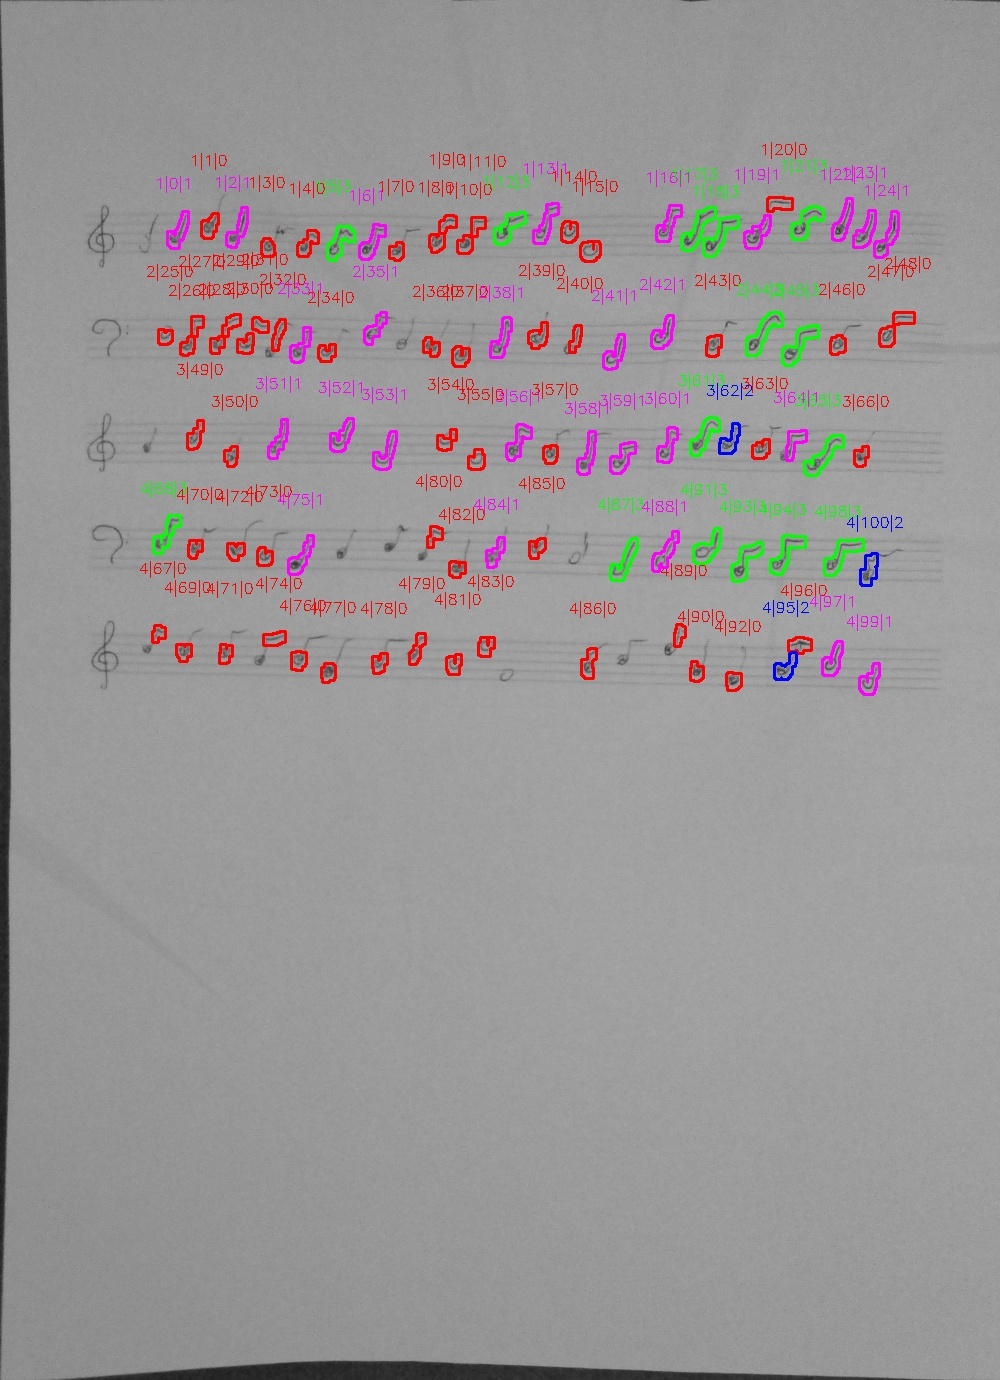
\includegraphics[width=\linewidth]{28_cnts.jpg}
        % \caption{Erozja}
        \label{fig:sub2}
    \end{subfigure}
    % \caption{Obraz oryginalny i po wycięciu}
    \label{fig:test}
\end{figure}

\begin{figure}[H]
    \centering
    \begin{subfigure}{.5\textwidth}
        \centering
        \graphicspath{ {Resources/} }
        \includegraphics[width=\linewidth]{nutki_30.jpg}
        % \caption{Threshold}
        \label{fig:sub1}
    \end{subfigure}%
    \begin{subfigure}{.5\textwidth}
        \centering
        \graphicspath{ {blobs/} }
        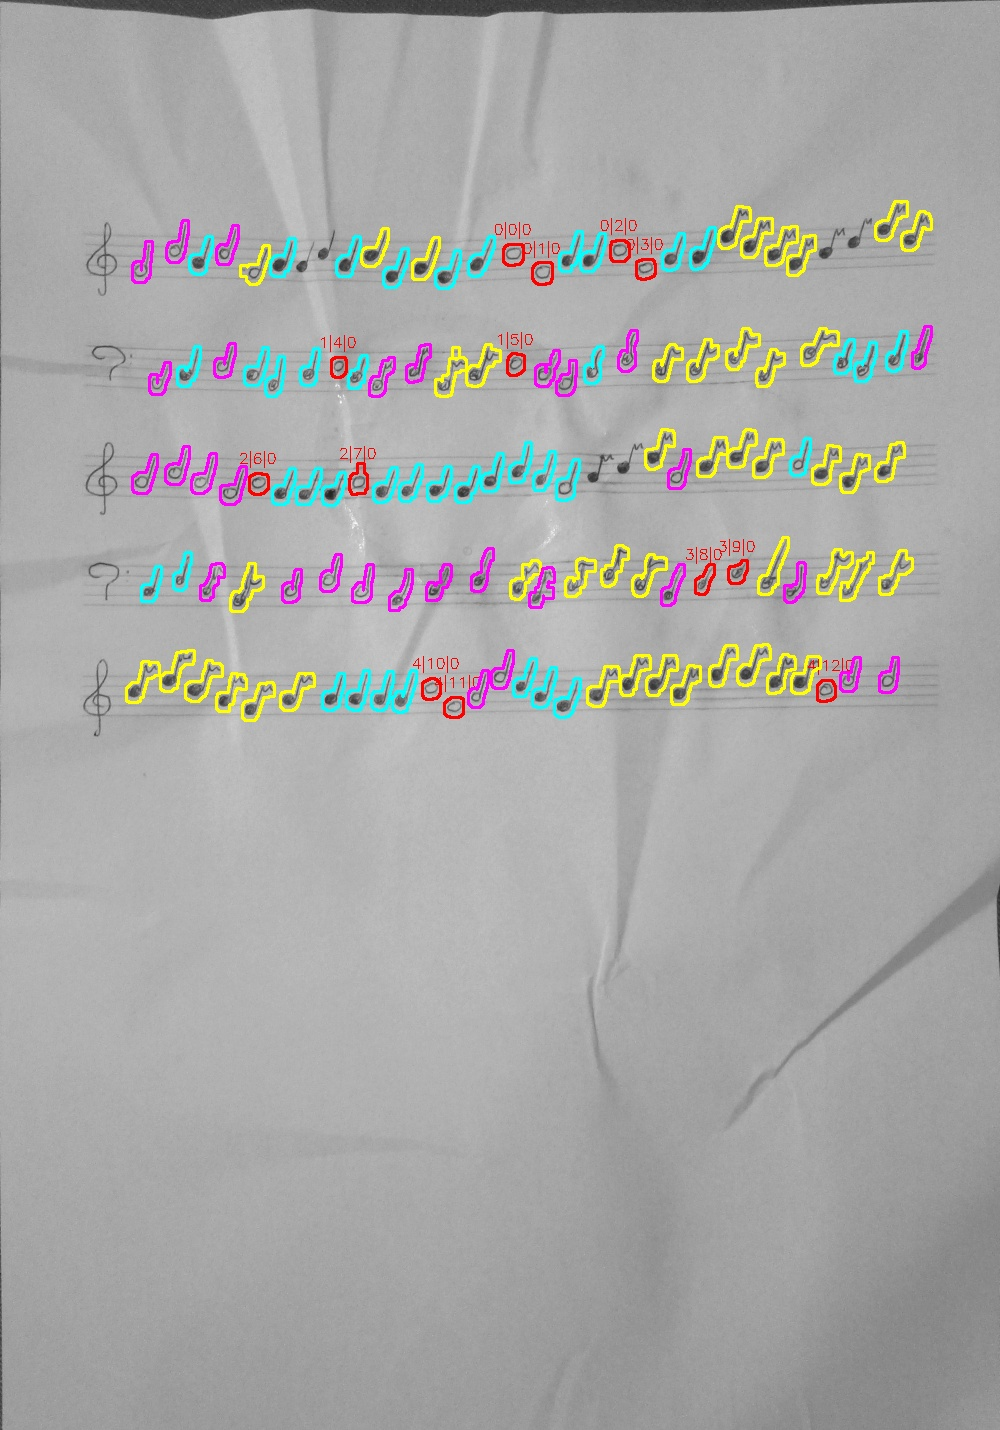
\includegraphics[width=\linewidth]{30_cnts.jpg}
        % \caption{Erozja}
        \label{fig:sub2}
    \end{subfigure}
    % \caption{Obraz oryginalny i po wycięciu}
    \label{fig:test}
\end{figure}

\begin{figure}[H]
    \centering
    \begin{subfigure}{.5\textwidth}
        \centering
        \graphicspath{ {Resources/} }
        \includegraphics[width=\linewidth]{nutki_31.jpg}
        % \caption{Threshold}
        \label{fig:sub1}
    \end{subfigure}%
    \begin{subfigure}{.5\textwidth}
        \centering
        \graphicspath{ {blobs/} }
        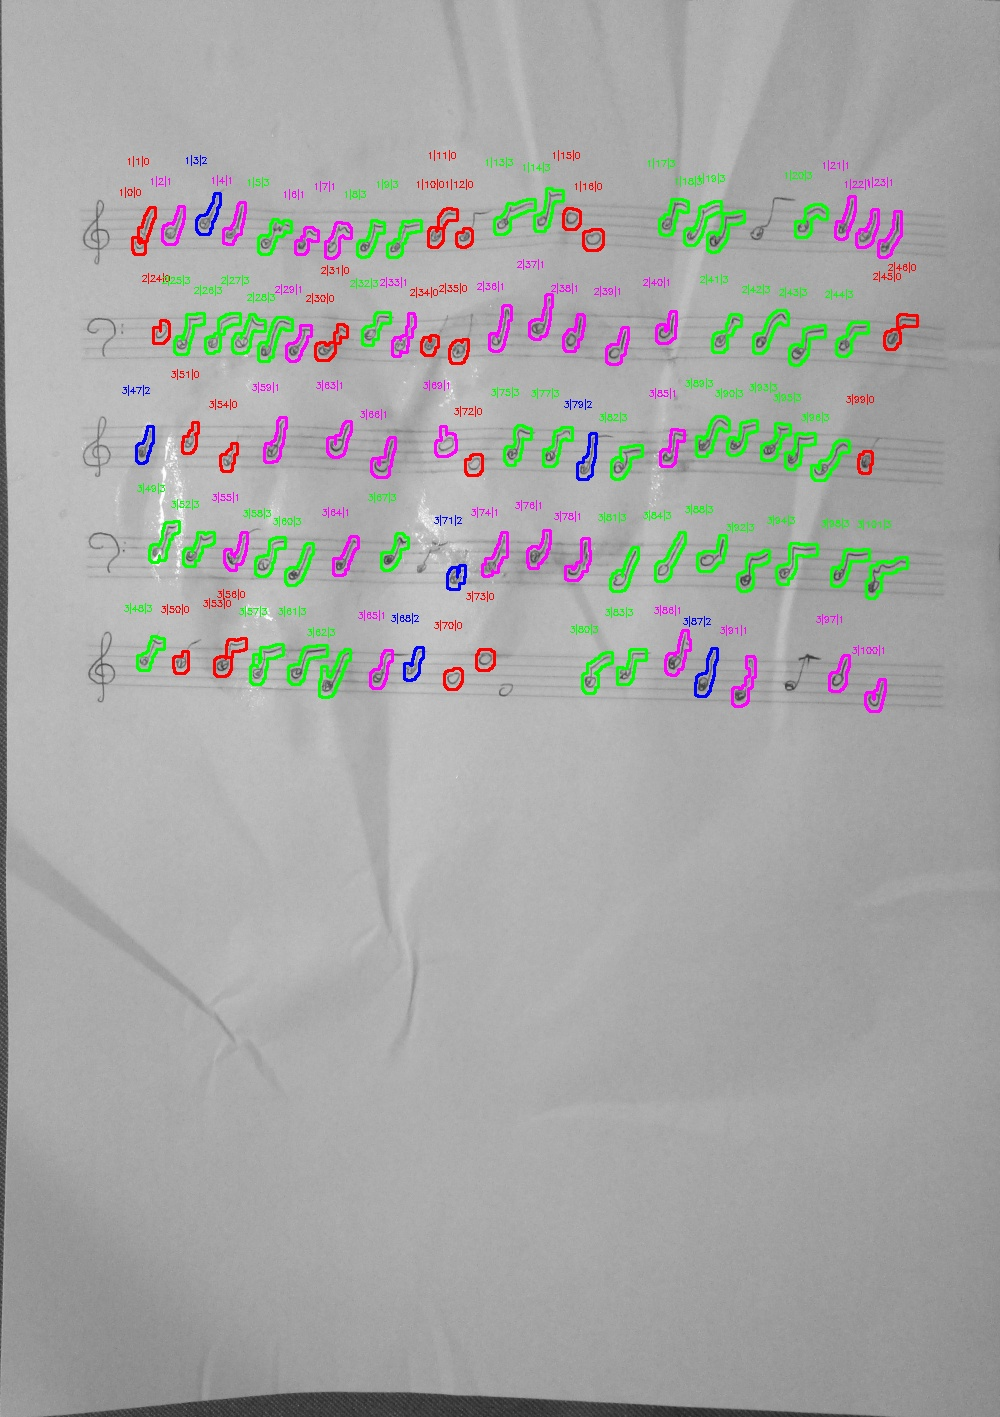
\includegraphics[width=\linewidth]{31_cnts.jpg}
        % \caption{Erozja}
        \label{fig:sub2}
    \end{subfigure}
    % \caption{Obraz oryginalny i po wycięciu}
    \label{fig:test}
\end{figure}


\end{document}